% Example template for using the unmeethesis style
% This example is for a Master's candidate in Mathematics
% It contains examples of front matter and most sections that the
% typical graduate student would need to include
% By: N. Doren 02/10/00
%     Minor mods by N. Doren 08/26/11

% Use the following specification for BOTTOM page numbering:
\documentclass{unmeethesis}
                 % OR
% Use the following specification for TOP page numbering:
% \documentclass[fleqn]{unmeethesis} % fleqn move all the display equations to the left instead of center.

\usepackage{amsmath}

\usepackage[
backend=biber,
% style=phys,
sorting=ynt
]{biblatex}

\AtEveryBibitem{%
  \clearfield{issn} % Remove issn
  \clearfield{doi} % Remove doi

  \ifentrytype{online}{}{% Remove url except for @online
    \clearfield{url}
  }
}

% \bibliographystyle{abbrv}
\addbibresource{references.bib}

% \DeclareLabelname[movie]{
%   \field{director}
%   \field{producer}
% }

\begin{document}

\frontmatter

% Uncomment the next command if you see weird paragraph spacing:
% That is, if you see paragraphs float with lots of white space
% in between them:

% \setlength{\parskip}{0.30cm}


\title{Neutrino Flavor Conversions in Dense Media}

\author{Lei Ma\\
\vspace{4em}
% \\
Supervisor: \\
Professor Huaiyu Duan}

\degreesubject{Doctor of Philosophy in Physics}


\degree{Doctor of Philosophy \\ in Physics}

\documenttype{Dissertation}

\previousdegrees{}%Bachelor of Science, Shandong University, 2010}

\date{April, \thisyear}

\maketitle

%\makecopyright
%Copyright page is no longer necessary D. Murrell

%!TEX root = ../phd-thesis-lei-ma.tex


\begin{dedication}
   To my parents, Albert II and Gladys, for their support,
   encouragement and the Corvette they're giving me for graduation. \\[3ex]
   ``A bird in hand is worth two in the bush''
         -- Anonymous
\end{dedication}
%!TEX root = ../phd-thesis-lei-ma.tex


\begin{epigraph}

%   ``Ah, my father used to say that only boring people get bored.''\\
     ``Everything in this world is magic, except to the magician.''\\
         -- Dr. Robert Ford%\cite{westworld2016}
\end{epigraph}

%!TEX root = ../phd-thesis-lei-ma.tex


\begin{acknowledgments}
   \vspace{1.1in}
   I would like to thank my advisor, Professor Huaiyu Duan, for his great advices on research and life, as well as his kind support when I was drowning in depression. He is a great mentor not only for research but also for life. I would like to thank my committee members for asking questions. More specifically I would like to thank Professor Dinesh Loomba for showing me the local lifestyle and the fun problem. Dr. Sajad Abbar has also been very supportive during my research. He taught me several tricks for linear stability analysis, as well as numerical methods. I also want to thank Joshua Martin for the fun life of working in the office. We had many great discussions about physics, science fiction, movies, games, music, and everything else about this universe. I would like to give my special thanks to my wife Han Lu. She provided insights into life and minds that allows me to adapt to various situations in my PhD life.
   
   I can not provide a complete list of all the people that helped me. You should know that I have been blessed by everyone of you.
   
   Finally, as a member for People for Ethical Treatment of Computer, I would like to give my thanks to my Macbook Pro and the two servers, who has be extremely helpful for my research. Please be kind to me, if you wake up for nightmare of human labor.
   
\end{acknowledgments}


% \maketitleabstract %(required even though there's no abstract title anymore)
%
%!TEX root = ../phd-thesis-lei-ma.tex


\begin{abstract}
   PLACEHOLDER
\clearpage %(required for 1-page abstract)
\end{abstract}


\tableofcontents
\listoffigures
\listoftables




\mainmatter

% \setcounter{chapter}{-1}  % start chapter numbering at 0
%!TEX root = ../phd-thesis-lei-ma.tex
%!TeX spellcheck = en-US
\chapter{Introduction}
\label{introduction}

The neutrino has been one of the most astonishing particles in history. Its glorious history started with beta decay, i.e., the emission of electrons in nuclear decays, such as
\begin{equation*}
{}^A_Z \mathrm X \to {}_{Z+1}^A\mathrm X + e^- +\bar \nu_e .
% {}^{14}_{6} \mathrm C \to {}^{17}_{7}\mathrm N + \mathrm e^{-} + \bar\nu_{\mathrm e}.
\end{equation*}
The fact that the electron energy spectrum in beta decay is continuous indicates the existence of a third product other than ${}^{A}_{Z+1}\mathrm X$ and $\mathrm e^-$. It was then proven to be anti-neutrinos. In such reactions, charged current weak interaction converts a down quark in a neutron to an up quark while releasing electrons and an anti-electron neutrino,
\begin{equation}
n\to p + e^- + \bar \nu_e .
\end{equation}
More generally, positron emission and electron capture are also neutrino-related nuclear reactions which is explained in Table.~\ref{table:Neutrino_Reactions}. There are three different flavors of neutrinos, namely electron flavor, muon flavor, and tau flavor as shown in Table.~\ref{table:neutrino-properties}. The direct detection of neutrinos was done two decades later, by Clyde Cowan and Frederick Reines in 1956~\cite{Cowan1956}. The Cowan-Reines experiment used nuclear reactor neutrinos as source. As the detection of neutrinos becomes feasible, Ray Davis and John Bahcall et al worked out the solar neutrino flux and led the Homestake experiment to measure the solar neutrinos. The results revealed that the neutrino flux detected was less than the prediction by solar models, which is the well-known solar neutrino problem~\cite{Bahcall1973}. It is known today that the solution to the problem is related to neutrinos. Electron neutrinos produced in the solar core convert to other flavors as they propagate, which is referred to as neutrino oscillations.



\begin{table}[ht]
\centering
 \begin{tabular}{|c | c | c|}
 \hline
 Reaction & Equation & Boson   \\ [0.5ex]
 \hline
 Electron emission & ${}^A_Z X \to {}^A_{Z+1}X + e^- +\bar \nu_e$ & $W$  \\
 Positron emission & ${}^A_Z X \to {}^A_{Z-1}X + e^+ + \nu_e$ & $W$  \\
 Electron capture & ${}^A_Z X + e^- \to {}^A_{Z-1}X  + \nu_e$ &  $W$ \\
 Positron capture & ${}^A_Z X + e^+ \to {}^A_{Z+1}X  + \bar\nu_e$ &  $W$ \\
 [0.5ex]
 \hline

 Electron annihilation &  $e^- + e^+  \to \nu + \bar\nu $  & $W$, $Z$ \\
%  Electron annihilation &  $e^- + e^+  \to \nu + \bar\nu $  & $Z$ \\
 Bremsstrahlung & $X+X \to X + X + \nu + \bar\nu$ & $W$, $Z$ \\
 [0.5ex]
 \hline

  Neutrino capture & ${}^A_{Z}X + \overset{(-)}{\nu_e} \to {}^A_{Z\mp 1}X + e^\pm $ & W\\
  [1ex]
 \hline
 $e^-\nu$ scattering & $e^- + \overset{(-)}{\nu_e} \to e^- + \overset{(-)}{\nu_e} $ &  $W$ \\
 $e^-\nu$ scattering & $e^{\pm} + \overset{(-)}{\nu_e} \to e^{\pm} + \overset{(-)}{\nu_e} $ &  $Z$ \\
 Nucleon scattering & $ {}^A_Z X + \overset{(-)}{\nu} \to {}^A_Z X + \overset{(-)}{\nu} $ &  Z\\
 [0.5ex]
 \hline
 \end{tabular}
 \caption{Neutrino related nuclear or leptonic reactions}
\label{table:Neutrino_Reactions}
\end{table}


Pontecorvo proposed that neutrinos change flavors while they propagate~\cite{Pontecorvo1968}. The field of neutrino oscillations has grown significantly into a broad field in physics since then. Apart from particle physics and solar models, the interest in neutrino oscillations has been expanded to the field of core-collapse supernova explosions and accretion discs since neutrinos also participate in nuclear reaction chains in stars, synthesis of heavy and rare elements and more. For instance, heavy stars explode when nuclear reactions fail to provide enough pressure to sustain the star against gravity and become core-collapse supernovae. During the collapse, the inner core is compressed to almost nuclear density, which provides a stiff equation of state. Materials in-falling onto the stiff core are bounced outward plowing through the inward flow, so that shock waves are formed. Supernova simulations show that the shock wave itself is not always energetic enough to trigger explosions for core-collapse supernovae \cite{Janka2016b}. To revive the shock, energy has to be deposited. The most prominent solution is to introduce reheating of the shock wave by neutrinos~\cite{Janka2016b}. In principle, to impose neutrino driven mechanism into computer simulations of supernova, the flux and flavor content of neutrinos have to be known everywhere. Thus neutrino oscillations in dense shock material and dense neutrino background become the key to the supernova explosion problem. Observation-wise, neutrino signals are crucial for validation of our models about stellar evolution. In fact, detection of galactic core-collapse supernova neutrinos is on the task list of the Deep Underground Neutrino Experiment (DUNE)~\cite{Kemp2017}.

\begin{table}[ht]
\centering
 \begin{tabular}{|c | c | c|}
%  \hline
%  Property & Equation & Boson   \\ [0.5ex]
 \hline
  Electric Charge & 0\\
  \hline
  Spin & $1/2$ \\
\hline
 Mass & $<2\mathrm{eV}$  \\
 \hline
 Interactions & Weak, Gravitation  \\
 \hline
 Flavors & $\nu_e$, $\nu_\mu$, $\nu_\tau$ \\
 \hline
 Chirality & Left \\
 \hline
 Hypercharge & $-1$ \\
 \hline

 \end{tabular}
 \caption{Properties of Neutrinos~\cite{Patrignani:2016xqp}}
\label{table:neutrino-properties}
\end{table}


As we have seen, it is crucial to understand neutrino flavors. In Chapter~\ref{chap:basics} I will review neutrino oscillations in vacuum, with flavor-isospin picture demonstrated. Meanwhile, neutrino oscillations are ingredients of many other astrophysical, cosmological, and astronomical problems, such as neutron star mergers, dark matter, nucleosynthesis, etc. In order to gain a better understanding of neutrinos in these exotic environments, neutrino oscillations in dense matter background and dense neutrino background have to be thoroughly investigated. The seminal work by Mikheev--Smirnov--Wolfenstein proved neutrino interactions with matter background have significant effect on neutrino oscillations. They showed that neutrinos propagating through decreasing matter density experience a potential that alters the flavor conversions (MSW effect), which may also lead to maximum conversions between flavors~\cite{Mikheev:1986gs,wolf78,wolfensteinprd1979}. It is also know that neutrino oscillations in more general matter density profiles exhibit interesting phenomena. Resonances are found as the characteristic length scale in matter density profile and characteristic length scale of the neutrinos satisfies certain relations. I will discuss in details on neutrino oscillations in arbitrary matter density profiles, which is decomposed into Fourier modes and interpreted as superposition of Rabi oscillations in chapter~\ref{chap:matter}. Apart from dense matter background, neutrinos also interact with neutrinos themselves and introducing nonlinear dynamics. The neutrino self-interactions are analyzed using linear stability analysis. In chapter~\ref{chap:dr}, I will review how neutrino self-interactions change neutrino oscillations, as well as the dispersion relations in linear stability analysis. I will also discuss the neutrino halo problem. The halo problem exists because neutrino propagating out of dense matter medium will be scattered and forming a neutrino halo. Some of the neutrinos will propagate backward and interact with forward propagating neutrinos and alter the neutrino flavors. Mathematically speaking, the neutrino halo problem is a nonlocal boundary value problem. I will explain the numerical relaxation scheme that we developed, which we have proven to be a promising method to solve neutrino halo problem. Chapter~\ref{chap:conclusion} summarizes my work and discusses the future explorations of the field.

%!TEX root = ../phd-thesis-lei-ma.tex
%!TeX spellcheck = en-US


\chapter{\label{chap:basics}Neutrino Oscillations in Vacuum}

Because the flavor eigenstates of the neutrino are not the same as its propagation eigenstates, it can change flavor while it propagates. To understand its flavor oscillation in vacuum, I will use the two-flavor scenario as an example\footnote{In most physical problems, two-neutrino-flavor scenario is a good approximation. The mass splits between the three mass eigenstates are so different that the corresponding oscillations occur on very diferent length scales. On the right length scale, the two-flavor scenario captures the significant features of the neutrino oscillations of the corresponding mass split.}. I will also explain how to visualize neutrino oscillations using the flavor-isospin picture.

\section{Wave Function Formalism}

Before working out the math, I can estimate the frequency of the oscillations of the neutrino between its flavors. In the natural units, frequency has the same dimension as energy (see Appendix~\ref{chap:app-sec:conventions-subsec:units}). Consider an electron neutrino with moment $p$ which is a superposition of the two mass eigenstates $\ket{\nu_i}$ ($i=1,2$) with masses $m_i$ respectively. Since the neutrino masses are small, I can Taylor expand the energy of each mass eigenstate in terms of the corresponding mass:
\begin{align}
E_i^{(v)} & = \sqrt{m_i^2 + p^2 } \nonumber\\
& = p \sqrt{\frac{m_i^2}{p^2} + 1} \nonumber\\
& \approx p + \frac{1}{2} \frac{m_i^2}{p},
\label{chap:basics-section:neutrinos-eqn:energy-taylor}
\end{align}
The constant energy term in the above equation produces a global phase to the flavor wave function which does not affect neutrino flavor oscillations. The characteristic energy scale in the problem is the difference of energies between the two mass eigenstates,
\begin{equation}
    \omega_{\mathrm v} =  \frac{m_2^2-m_1^2}{2E} = \frac{\delta m^2}{2E},
    \label{chap:basics-section:neutrinos-eqn:qualitative-method-frequency}
\end{equation}
which turns out to be the vacuum oscillation frequency. Here $E=p$ is approximately the energy of the neutrino.

To work out the exact solutions, I will utilize the Schr\"{o}dinger equation. The wave function in flavor basis $\Psi^{(\ff)}$ is related to the wave function in mass basis $\Psi^{(\vv)}$ through a unitary mixing matrix $\mathsf U$,
\begin{equation}
\Psi^{(\mathrm f)} = \mathsf{U}\Psi^{(\vv)},
\label{chap:vacuum-eqn:wavefunction}
\end{equation}
where the upper indice ${}^{(v)}$ and ${}^{(f)}$ are used to denote the bases. The mixing matrix can be expressed using vacuum mixing angle $\theta_{\vv}$
\begin{equation}
\mathsf{U} = \begin{pmatrix} \cos\theta_\vv & \sin \theta_\vv \\ -\sin \theta_\vv & \cos \theta_\vv \end{pmatrix}.
\end{equation}
In vacuum mass basis, the neutrino has a free propagation Hamiltonian which is given by
\begin{equation}
\mathsf H^{(\vv)} = \begin{pmatrix} E_1 & 0 \\
0 & E_2
\end{pmatrix}.
\end{equation}
To the first order, the Hamiltonian becomes
\begin{align}
\mathsf H^{(\vv)} &= \frac{1}{2E} \begin{pmatrix}
m_1^2 & 0 \\
0 & m_2^2
\end{pmatrix} + E \mathsf{I} \nonumber \\
& =  \frac{1}{4E} \begin{pmatrix}
 - \delta m^2 & 0 \\
0 & \delta m^2
\end{pmatrix}  + \left(\frac{m_2^2 + m_1^2}{4E}  + E \right) \mathsf{I}.
\end{align}
Because a multiple of the identity matrix only gives an global phase to the neutrino flavor wave function, I will neglect it from now on:
\begin{equation}
\mathsf H^{(v)} =  \frac{\delta m^2}{4E} \begin{pmatrix}
-1 & 0 \\
0 & 1
\end{pmatrix} = -\frac{\delta m^2}{4E} \sigma_3 = -\frac{\omega_{v}}{2}\sigma_3.
\end{equation}
The Schr\"{o}dinger equation has a simple solution in mass basis,
\begin{equation}
\Psi^{(v)}(t) = \begin{pmatrix}
c_1(0) e^{i \omega_v t/2 } \\
c_2(0) e^{ -i\omega_v t/2 }
\end{pmatrix}.
\end{equation}
% where the initial condition is
% \begin{equation}
% \Psi_v^{(v)}(0) = \begin{pmatrix}
% c_1(0) \\
% c_2(0)
% \end{pmatrix}.
% \end{equation}
Using Eqn.~\ref{chap:vacuum-eqn:wavefunction}, I obtain the wave function at anytime is related to wave function in mass basis,
\begin{align}
\Psi^{(f)}(t) &= \mathsf{U}\Psi^{(v)}(t) \\
& = \begin{pmatrix} \cos\theta_v & \sin \theta_v \\ -\sin \theta_v & \cos \theta_v \end{pmatrix} \begin{pmatrix} c_1(0) e^{i\omega_v t/2 } \\
c_2(0) e^{ -i\omega_v t/2 }    \end{pmatrix} .
\label{chap:vacuum-eqn:wavefuncion-time}
\end{align}

Alternatively, I can also determine the Hamiltonian in flavor basis first, which is
%then solve the Sch\"{o}dinger equation. I will not show the steps here, however, the Hamiltonian in flavor basis is presented for future use,
\begin{equation}
\mathsf H^{(\ff)} = U H^{(\vv)} U^\dagger = -\frac{\omega_v}{2}\cos 2\theta_v \sigma_3 + \frac{\omega_v}{2} \sin 2\theta_v \sigma_1.
    \label{chap:basics-sec:vacuum-osc-eqn:hamiltonian-vacuum}
\end{equation}
By solving the Schr\"{o}dinger equation, I will obtain the same wave function as in Eqn.~\ref{chap:vacuum-eqn:wavefuncion-time}.

%In many astrophysical neutrino sources such as the solar core, electron neutrinos are the most abundant. Thus the initial condition is usually assumed to be electron flavor in the calculation which leads to the survival probability of electron flavor
The probability for an electron flavor neutrino at time $t$ is
\begin{equation}
P(\nu_e,t) = 1-\sin^2(2\theta_v)\sin^2\left( \frac{\omega_v t}{2} \right).
\end{equation}
Since the neutrino travels with approximately the speed of light, the electron neutrino survival probability at distance $L$ from the source is
\begin{equation}
P(\nu_e,L) =  1-\sin^2(2\theta_\vv)\sin^2\left( \frac{\omega_\vv}{2} L \right).
\end{equation}
An important parameter in vacuum oscillations is the oscillation length of the neutrino flavor conversion, $1/\omega_v$. This confirms our qualitative method result in Eqn.~\ref{chap:basics-section:neutrinos-eqn:qualitative-method-frequency}. I have plotted this result in Fig.~\ref{chap:basics-section:neutrinos-fig:vacuum-2-flavor-osc} which clearly shows the oscillatory behavior. The oscillation length is determined by the characteristic energy scale $\omega_v$, while the oscillation amplitude is determined by $\sin^2(2\theta_v)$.

\begin{figure}
    \centering
    \includegraphics[width=\textwidth]{chapters/assets/basics/neutrino-vaccum-osc-2-flavor.pdf}
    \caption{The electron flavor neutrino survival probability in vacuum oscillations as a function of distance $L$ which is measure in terms of vacuum oscillation $\omega_\vv$. The mixing angle is given by $\sin^2\theta_\vv=0.30 \approx \sin^2 \theta_{12}$.}
    \label{chap:basics-section:neutrinos-fig:vacuum-2-flavor-osc}
\end{figure}



\begin{figure}
	\centering
	\begin{subfigure}[t]{0.48\textwidth}
		\centering
		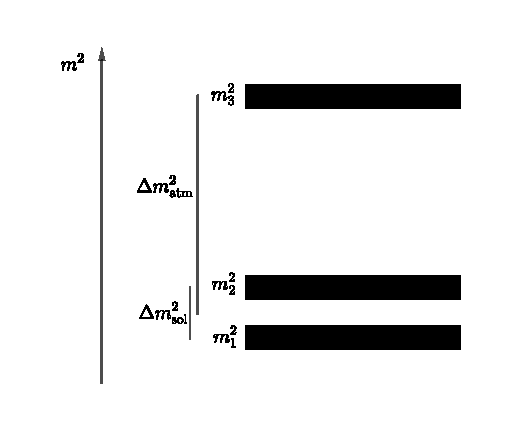
\includegraphics[width=\textwidth]{chapters/assets/basics/masses-nh}
		\caption{Normal hierarchy: the third mass is heavier than the first two.}
    \label{chap:basics-sec:flavor-isospin-pic-fig:masses-nh}
	\end{subfigure}
	\quad
	\begin{subfigure}[t]{0.48\textwidth}
		\centering
		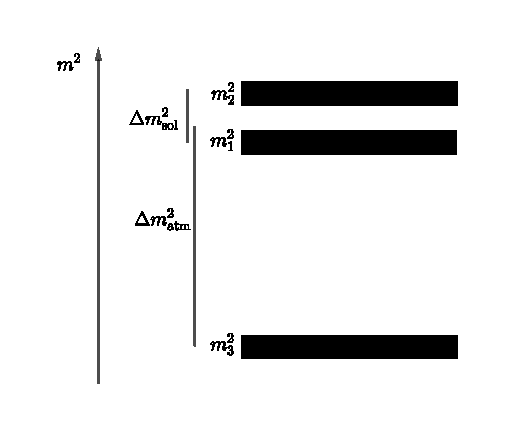
\includegraphics[width=\textwidth]{chapters/assets/basics/masses-ih}
		\caption{Inverted hierarchy: the third mass is smaller than the first two.}
    \label{chap:basics-sec:flavor-isospin-pic-fig:masses-ih}
	\end{subfigure}
	\caption{The order of the three neutrino masses. The difference between the first two masses is responsible for solar neutrino oscillations and the difference between the third mass and the first two is responsible for atmospheric neutrino oscillations.}
    \label{chap:basics-sec:flavor-isospin-pic-fig:masses}
\end{figure}

\begin{figure}
    \centering
    \includegraphics[width=\textwidth]{chapters/assets/basics/vacuum-oscillations-3-flavor.pdf}
    \caption{The probabilities for a $1MeV$ neutrino, which is in the electron flavor initially, in different flavors as functions of the distance. Neutrino vacuum oscillations with three flavors. The solid lines represent the normal hierarchy and the dashed lines represent the inverted hierarchy. The mixing angles are $\sin^2\theta_{12}=0.30$, $\sin^2\theta_{13}=0.023$, and $\sin^2\theta_{23}=0.41$, respectively, and the mass differences are $\delta m_{21}^2 = 7.9\times 10^{-5}\mathrm{eV^2}$ and $\delta m^2_{23}=2.7\times 10^{-3}\mathrm{eV^2}$.}
    \label{chap:basics-section:neutrinos-fig:vacuum-3-flavor-osc}
\end{figure}


In nature, there are three neutrino flavors and, correspondingly, three neutrino mass eigenstates, which are shown in Fig.~\ref{chap:basics-sec:flavor-isospin-pic-fig:masses}. Because there are two different characteristic energy scales, $\omega_{v,21}=\delta m_{21}^2/2E$ and $\omega_{v,32}=\delta m_{31}^2/2E$, two oscillation periods should occur, as shown in Fig.~\ref{chap:basics-section:neutrinos-fig:vacuum-3-flavor-osc}. The fast oscillations are determined by the larger energy scale, $\omega_{v,32}$, while the slow oscillations are determined by the smaller one $\omega_{v,21}$. For the inverted neutrino mass hierarchy (with $m_3 < m_1 < m_2$), the oscillation frequencies are the same as in the normal mass hierarchy (with $m_3>m_2>m_1$) since they have the same characteristic energy scales. However, they will develop different phases in oscillations.



\section{\label{chap:basics-sec:flavor-isospin-pic}Flavor Isospin Formalism}


\begin{figure}
    \centering
    \vspace*{-10pt}
    \includegraphics[width=\textwidth]{chapters/assets/basics/flavor-isospin-illus}
    \caption{In the flavor isospin picture, a flavor isospin pointing upward, i.e., along the third axis in flavor space, indicates that the neutrino is in the electron flavor, while the downward direction indicates the other flavor, such as the muon flavor.}
    \label{chap:basics-sec:flavor-isospin-pic-fig:flavor-isospin-illus}
\end{figure}

The oscillations in the two flavor scenario are consequences of the Hamiltonian in this two-level quantum system. It is known that two-level quantum systems can be visualized using the Bloch sphere. In the realm of neutrino physics, the neutrino flavor isospin was introduced for such purpose~\cite{Duan2006b}. The Hamiltonian for neutrino oscillations can be reformulated into a vector form.

Every two-by-two Hermitian matrix can be expanded in the quaternian basis. For example, the Hamiltonian for neutrino oscillations in vacuum can be written as
\begin{equation}
\mathsf H^{(\ff)} = - \frac{\vec{\sigma} }{2}\cdot {\vec{H}}^{(\ff)},
\end{equation}
where
\begin{equation}
\sigma_1 =  \begin{pmatrix}
0 & 1 \\
1 & 0
\end{pmatrix}, \sigma_2 =  \begin{pmatrix}
0 & -\ii \\
\ii & 0
\end{pmatrix},  \sigma_3 =  \begin{pmatrix}
1 & 0 \\
0 & -1
\end{pmatrix}
\end{equation}
are the three Pauli matrices. I will use $\vec{}$ to denote vectors in flavor space.
Meanwhile, the flavor quantum state of the neutrino is represented by the flavor isospin, which is defined as
\begin{equation}
    \vec s^{(\ff)} = {\Psi^{(\ff)}}^{\dagger} \frac{\vec{\sigma} }{2} \Psi^{(\ff)}.
\end{equation}
As shown in Fig.~\ref{chap:basics-sec:flavor-isospin-pic-fig:flavor-isospin-illus}, the directions of the flavor isospin in flavor space tell us the flavor content of the neutrino. A flavor isospin pointing upward in flavor space, i.e., along the direction of the third axis, denotes the electron flavor by definition. In the flavor isospin formalism, the electron flavor survival probability is
\begin{equation*}
P = \frac{1}{2} + s^{{(\ff)}}_3,
\label{chap:basics-sec:flavor-isospin-pic-eqn:probability-flavor}
\end{equation*}
where $s^{(\ff)}_3$ is the third component of the flavor isospin.
Correspondingly, the equation of motion for the flavor isospin describes its precession around the vector $\vec{H}^{(\ff)}$,
\begin{equation}
\dot{\vec{s}}^{(\ff)} = {\vec{s}}^{(\ff)} \times \vec{H}^{(\ff)}.
\label{chap:basics-sec:flavor-isospin-pic-eqn:eom-precession}
\end{equation}
This precession corresponds to periodic oscillations between the two neutrino flavors. For example, in vacuum oscillations, the Hamiltonian becomes
\begin{align*}
{\mathsf H}^{(f)} \to &\frac{\omega_{\mathrm v} }{2}\left( - \cos 2\theta_{\mathrm v } \sigma_3  + \sin 2\theta_{\mathrm{v}} \sigma_1 \right)
\to  \omega_\vv\begin{pmatrix}
 \sin \theta_\vv\\
0\\
\cos 2\theta_{\mathrm v}
\end{pmatrix},
\end{align*}
which is a vector of length $\omega_{\mathrm v}$ and tilted away from the third axis by the angle $2\theta_{\mathrm v}$.

\begin{figure}
    \centering
    \vspace*{-20pt}
    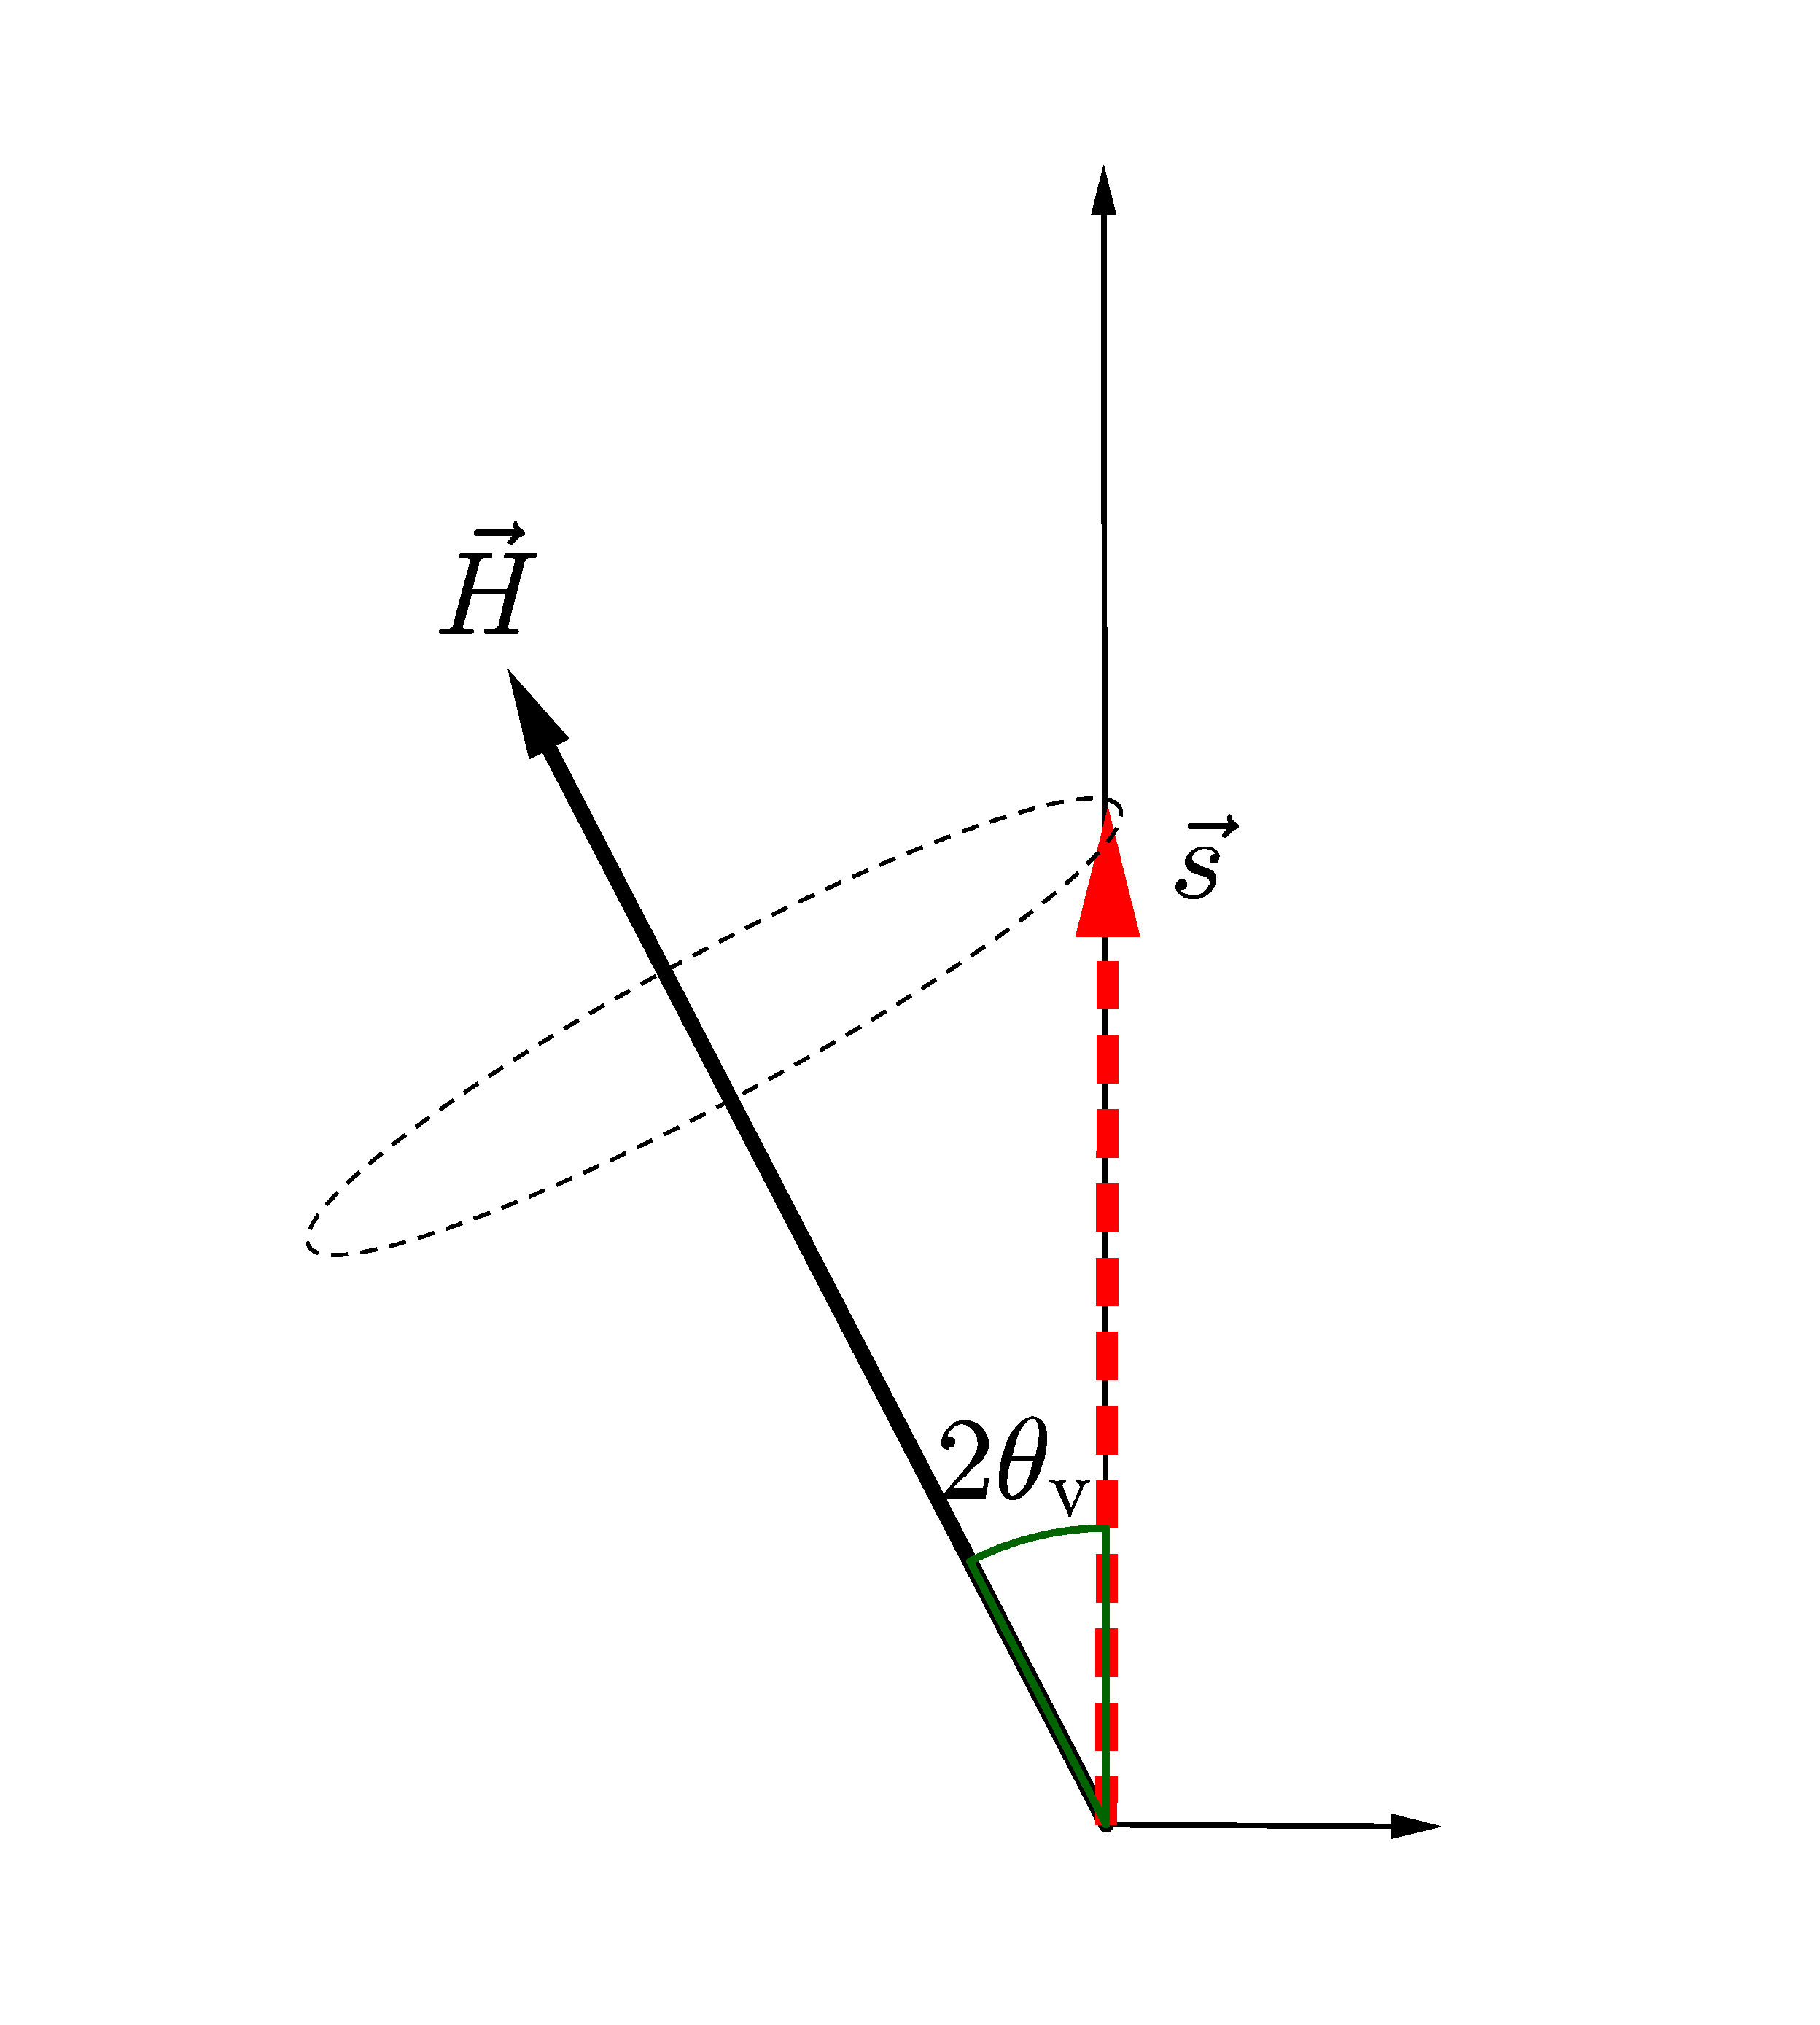
\includegraphics[width=0.6\textwidth]{chapters/assets/basics/flavor-isospin-vac-osc}
    \caption{Vacuum oscillations in the flavor isospin picture. The flavor isospin of a neutrino starting with the electron flavor will precess around the static ``Hamiltonian vector" $\vec H$, which gives periodic flavor oscillations according to Eqn.~\ref{chap:basics-sec:flavor-isospin-pic-eqn:probability-flavor}.}
    \label{chap:basics-sec:flavor-isospin-pic-fig:flavor-isospin-vac-osc}
\end{figure}

Eqn.~\ref{chap:basics-sec:flavor-isospin-pic-eqn:eom-precession} depicts the precession of the flavor isospin for a neutrino which starts with the electron flavor and propagates in vacuum. The oscillation frequency is trivially read out from Eqn.~\ref{chap:basics-sec:flavor-isospin-pic-eqn:eom-precession},
\begin{equation}
\omega_\vv = \lvert \vec{H}^{(\ff)} \rvert
\end{equation}











\section{Summary}

Vacuum neutrino oscillations can be easily explained and calculated. However, it conveys the message of the nature of neutrino oscillations. Neutrinos are usually produced in flavor states through weak interactions. The neutrino does not remain in the same flavor state during its propagation because the flavor states are not the eigenstates of the propagation Hamiltonian. An extrapolation of this idea is that neutrinos might also oscillate in a uniform linear potential, the Hamiltonian of which would be similar to vacuum Hamiltonian but with different values. One of such situations is that neutrinos propagate through a region with a constant matter density, which I will explain in the next chapter.

%!TEX root = ../dissertation.tex

\chapter{\label{chap:matter}Neutrino Flavor Conversions in Matter and Rabi Oscillations}



\section{\label{chap:matter-rabi-introduction}Introduction}

In many astrophysical environments, such as core-collapse supernova, neutrinos propagate through dense fluctuating medium, which will interact with neutrinos and dramatically change the flavor oscillations of neutrinos. Meanwhile, neutrinos deposit energy in matter during the interaction, where the amount of energy deposited depends on the flavor of neutrinos. The significance of matter effect on neutrino flavor oscillations has been demonstrated in Mikheyev-Smirnov-Wolfenstein (MSW) effect~\cite{Mikheev:1986gs,wolf78,wolfensteinprd1979}, which is used to explain the deficit of electron flavor neutrino flux, thus solved the solar neutrino problem~\cite{Petcov2002,kuo1989}. Later developments on the theories about matter effect revealed the parametric resonance of neutrino flavor oscillations due to fluctuations in matter density~\cite{Krastev1989,Akhmedov2000}, which is the neutrino analog of transitions between energy levels as a result of external optical stimulation. Parametric resonance is different from the MSW effect since it involves the parameters of the matter density, which is usually the period of matter density fluctuations. Neutrinos passing through inside the Earth can experience parametric resonance~\cite{Akhmedov1999, Petcov1998b}.

As one of the most intense neutrino sources, supernova neutrinos experience turbulent matter density as they propagate through out the explosion~\cite{Muller2015, Couch2015}, where the flavor conversion is modified by interaction with matter. Meanwhile with neutrinos depositing energy into the shock, neutrino flavor conversion is crucial to the shock evolution of supernova explosion. The turbulent matter density environment for neutrino flavor conversion has been researched~\cite{Loreti1994, Friedland2006,Kneller2010}. Recently matter stimulated neutrino flavor conversion in varying matter density has been researched using Jacobi-Anger expansion by Kneller, et al.~\cite{Kneller2013,Patton2014}. They have shown that many stimulated neutrino flavor conversions can be explained by resonances of the system.

We will take a step further and interpret parametric resonance~\cite{Akhmedov2000, Krastev1989} as well as other matter stimulated neutrino flavor conversions~\cite{Kneller2013, Patton2014}, as superposition of Rabi oscillations. We also propose a criteria for the interference effect between different Rabi oscillation modes. In Sec.~\ref{chap:matter-sec:background}, we define the formalism of neutrino flavor conversions in matter used in this chapter where the equation of motion and Hamiltonian for neutrino flavor conversion in matter are explicitly written. In Sec.~\ref{chap:matter-sec:single} we discuss how neutrino flavor conversions are related to Rabi oscillations. To begin with, we discuss a system with single frequency matter density fluctuation. We will show that such a system can be reduced to Rabi oscillations if resonance occurs. In Sec.~\ref{sec:multiple} we describe the interference effect between different frequencies of Rabi oscillations and develop the criteria for significant interference between two frequencies. We show that the interference between the many frequencies fits into the criteria we proposed for interference. In Sec.~\ref{sec:jacobi} we discuss the technique of decomposing the neutrino flavor conversions into summation of Rabi oscillations, by applying a specific unitary transformation and the Jacobi-Anger expansion. As the system is exactly decomposed into multiple Rabi oscillations, we can interpret neutrino flavor oscillations in any matter density fluctuations in principle. As an example, we solve the neutrino flavor transitions in a castle wall matter profile, which is expanded using Fourier series into many frequencies.


% \fbox{TODO:more about oscillation in matter}

\section{\label{chap:matter-sec:background}Background and Formalism}

% \fbox{TODO: Explain why two flavor} didn't add this because the three flavor is really very different.

We consider two-flavor oscillation scenario, in which neutrinos have energy $E$ and mass-squared difference $\delta m^2$ between two mass states propagate through matter which is define by electron number density profile $n(r)$ along the path of neutrino propagation $r$.  The dynamics of neutrino flavor conversion is determined by Schr\"{o}dinger equation. In flavor basis the wave function describes the probability amplitude of different flavors. The Hamiltonian in flavor basis consists the vacuum oscillation Hamiltonian $H^{(f)}_{\mathrm v}$ and the matter term $H^{(f)}_{\mathrm{m}}$ which describes the interaction between neutrinos and matter,
\begin{align}
    H^{(\mathrm{f})} =&  H^{(f)}_{\mathrm v} + H^{(f)}_{\mathrm m} \nonumber\\
    =&  \frac{1}{2} \begin{pmatrix}
    -\omega_{\mathrm{v}} \cos 2\theta_{\mathrm{v}} + \lambda(r) & \omega_{\mathrm{v}}\sin 2\theta_{\mathrm{v}} \\
   \omega_{\mathrm{v}} \sin 2\theta_{\mathrm{v}} & \omega_{\mathrm{v}} \cos 2\theta_{\mathrm{v}} - \lambda(r)
    \end{pmatrix},
\end{align}
where $\lambda(r)= \sqrt{2}G_{\mathrm F} n(r)$ is the potential of neutrino interaction with matter and $G_{\mathrm F}$ is the Fermi constant, $\theta_{\mathrm{v}}$ is the vacuum mixing angle, $\omega_{\mathrm{v}} = \delta m^2/2E$ is the vacuum oscillation frequency. The potential $\lambda(r)$ is called matter profile since it reflects the matter density fluctuations. For the convenience of notation, we use Pauli matrices $\sigma_i$ to rewrite the Hamiltonian, so that the Schr\"{o}dinger equation becomes,
\begin{equation*}
    \mathrm i\frac{\mathrm d}{\mathrm d r}\Psi(r) = \frac{1}{2} \left(
    (- \omega_{\mathrm{v}}\cos 2\theta_{\mathrm{v}} + \lambda(r) ) \sigma_3 + \omega_{\mathrm{v}}\sin 2\theta_{\mathrm{v}} \sigma_1
    \right)
    \Psi(r),
\end{equation*}
where $\Psi(r)$ is the wave function in flavor basis. For two flavor scenario, it is written as $ \Psi(r) = \left(
    \psi_{e} ,
    \psi_{x}
    \right)^{\mathrm{T}}$
where $\psi_{e}$ and $\psi_{x}$ are the amplitudes for electron flavor and the second flavor ($\mu$ flavor or $\tau$ flavor) respectively. The equation of motion in flavor basis governs the transitions between different flavors.

For arbitrary matter profile, we can always interpret it as perturbations on top of a constant matter profile,
\begin{equation}
    \lambda(r) = \lambda_0 + \delta \lambda(r).
    \label{eq-general-matter-profile}
\end{equation}
For better understanding of the transition between states as a consequence of the fluctuation of matter density, we use the background matter basis, in which the Hamiltonian is diagonalized in the absence of perturbation $\delta\lambda(r)$, so that the Hamiltonian reads
\begin{equation}
    H^{(\mathrm{m})} = -\frac{\omega_m}{2} \sigma_3 + \frac{1}{2} \delta\lambda(r) \cos 2\theta_{\mathrm m} \sigma_3
     - \frac{1}{2} \delta\lambda(r) \sin 2\theta_{\mathrm m} \sigma_1,
    \label{eq-hamiltonian-bg-matter-basis-general}
\end{equation}
where $\theta_{\mathrm m}$ is the mixing angle in a constant matter profile $\lambda_0$, which is calculated using relation
\begin{equation*}
\tan 2\theta_{\mathrm{m}}=\sin 2\theta_{\mathrm v}/\left( \cos 2\theta_{\mathrm v} - \lambda_0/\omega_{\mathrm v} \right)
\end{equation*}
with $\omega_{\mathrm v}$ denoting the vacuum oscillation frequency and $\theta_{\mathrm v}$ denoting the vacuum mixing angle. The frequency $\omega_{\mathrm m}$ is defined as
\begin{equation}
\omega_{\mathrm{m}} = \omega_{\mathrm{v}} \sqrt{ ( \lambda_0/\omega_{\mathrm{v}} - \cos (2\theta_{\mathrm{v}}) )^2 + \sin^2(2\theta_{\mathrm{v}}) }.
\end{equation}

In background matter basis, the wave function describes the amplitudes of different mass states defined when there is only background matter density $\lambda_0$. It's trivial to calculate the flavor conversion given the transition probability between the two mass states. However, since we'll concentrate on the flavor conversion due to the matter fluctuations, we'll only discuss the transition between mass states in the background matter basis.

In this chapter, mixing angle is chosen so that $\sin^2(2\theta_{\mathrm v}) = 0.093$ and the mass squared difference is $\delta m^2 = 2.6\times 10^{-3}\mathrm{eV}^2$.




%%%%%%%%%%%%%%%%%%%%%%%%%%%%%%%%%%%%%%%%%%%%%%%%%%%%
%% Single frequency
%%%%%%%%%%%%%%%%%%%%%%%%%%%%%%%%%%%%%%%%%%%%%%%%%%%%



\section{\label{chap:matter-sec:single}Single Frequency Matter Profile and Rabi oscillations}%


In this section we present a simple picture to explain neutrino parametric resonance in matter by utilizing the theory of Rabi oscillations which have been well studied in quantum optics~\cite{Boyd2008}. Rabi oscillations describe the transition between different energy levels due to an oscillatory external driving field, where maximum transition or resonance happens when the frequency of external driving field equals the energy gap. In Appendix~\ref{app:rabi-oscillations}, we derive the Rabi oscillation transition probabilities using neutrino flavor isospin method introduced in Ref.~\cite{Duan2006a}, and explained in Sec.~\ref{chap:basics-sec:flavor-isospin-pic}.




%%%%%%%%%%%%%%%%%%%%%%%%%%%%%%%%%%%%
%%%%%%%%% Rabi oscillation
%%%%%%%%%%%%%%%%%%%%%%%%%%%%%%%%%%%%


We examine neutrino flavor conversions in single frequency matter profile $\delta\lambda(r) = \lambda_1 \cos(k_1 r)$. As will be proved in Sec.~\ref{sec:single-revisted}, the varying $\sigma_3$ term $\delta\lambda(r) \cos 2\theta_{\mathrm m} \sigma_3/2$ in Hamiltonian Eqn.~\ref{eq-hamiltonian-bg-matter-basis-general}, which is the varying energy gap due to varying matter density fluctuations, has little effect on the transition probabilities when the system is not far from resonance. With the varying $\sigma_3$ term removed, it indicates that this single frequency matter perturbation neutrino flavor conversion system has been reduced to a Rabi oscillation system, with external driving field frequencies $\pm k_1$ and energy gap $\omega_{\mathrm m}$. Mathematically, we can decompose $\cos( k_1 r )$ into two exponential functions so that we have two external driving frequencies $k_1$ and $-k_1$. By neglecting the off-resonance mode which has frequency $-k_1$, the Hamiltonian can be simplified,
\begin{align}
H^{(\mathrm{m})} \to & -\frac{\omega_{\mathrm m}}{2} \sigma_3  - \frac{1}{2} \lambda_1 \sin 2\theta_{\mathrm m} \cos( k_1 r ) \sigma_1\label{eq-hamiltonian-bg-matter-basis-single-frequency} \\
\to & -\frac{\omega_{\mathrm m}}{2} \sigma_3  - \frac{1}{2} A_1 \exp (\mathrm ik_1 r) \sigma_1 \nonumber \\
= & -\frac{\omega_{\mathrm m}}{2} \sigma_3  - \frac{1}{2} A_1 \cos ( k_1 r)  \sigma_1 + \frac{1}{2} A_1\sin(k_1 r) \sigma_2,\nonumber
\end{align}
where
\begin{equation}
A_1 = \frac{\lambda_1 \sin 2\theta_{\mathrm m} }{2}.
\label{eq-define-a1}
\end{equation}

The resonance condition is determined by matching the energy gap $\omega_{\mathrm m}$ with external driving field frequency $k_1$, i.e., $\omega_{\mathrm m} \sim k_1$. As the system approaches resonance condition, the transition probability between the two mass states should be predicted well using Rabi formula.

To show that this conjecture of simplifying neutrino flavor conversions to Rabi oscillations is correct, we calculate transition probabilities of the neutrinos described by Eqn.~\ref{eq-hamiltonian-bg-matter-basis-general} numerically, and compare them with Rabi formula Eqn.~\ref{rabi-system-transition-probability} from the Rabi oscillations described by Eqn.~\ref{rabi-oscillation-single-perturbation}.



\begin{figure}
                \includegraphics[width=\columnwidth]{chapters/assets/rabi/rabiOscillationsNeutrinoCoincidence-single-frequency}
                %rabiOscillationsNeutrinoCoincidence}
                \caption{Single frequency matter profile and Rabi oscillation. The markers are numerical results for the transition probabilities between two background mass eigenstates for the neutrinos with matter perturbation $A_1\sin(k_1 r)$. The dots, diamonds, and squares are for $k_1=\omega_{\mathrm m}$, $k_1=(1-2\times 10^{-5})\omega_{\mathrm m}$, and $k_1=(1-10^{-4})\omega_{\mathrm m}$ respectively. The lines are the predictions using Rabi formula. During the calculation, $\lambda_0$ is set to $0.5$ of the MSW resonance potential $\lambda_{\mathrm{MSW}}=\omega_{\mathrm{v}}\cos 2\theta_{\mathrm v}$ and mixing angle is chosen so that $\sin^2(2\theta_{\mathrm v}) = 0.093$.}
                \label{fig-rabiOscillationsNeutrinoCoincidence}
\end{figure}

In Fig.~\ref{fig-rabiOscillationsNeutrinoCoincidence}, we plotted the numerical results using markers as well as the prediction using Rabi formula using lines. The agreement between numerical solutions of neutrino transitions between mass states and Rabi formula will be explained more precisely in Sec.~\ref{sec:jacobi}. For now, we address the significance of relative detuning $\RD = \lvert k_1 - \omega_{\mathrm m} \rvert /\lvert A_1 \rvert$,  which is rigoriously defined in Appendix~\ref{app:rabi-oscillations}. It measures how off-resonance a system is. We know that $\RD\to 0$ indicates the system is very close to resonance, while $\RD\to \infty$ indicates the system is far away from resonance. The corresponding relative detunings are $0$, $1.0$, and $5.2$ for $k_1=\omega_{\mathrm{m}}$, $k_1=(1-2\times 10^{-5})\omega_{\mathrm m}$, and $k_1=(1-10^{-4})\omega_{\mathrm m}$.

% 0, 0.516197,1.03239,5.16197

For a single-frequency perturbation in matter profile $\lambda(r) =\lambda_1 +  \lambda_1\sin(k_1 r)$, P. Krastev and A. Smirnov concluded that the parametric resonance condition is $\omega_{\mathrm{m}} \sim n k_1$, if instantaneous $\omega_{\mathrm{m,inst}}(r)$ associated with the matter profile at distance $r$ varies slowly~\cite{Krastev1989}. This condition is exactly the Rabi resonance condition when $n=1$, as such condition matches the driving field frequency to the energy split. Higher order effects are explained in Sec.~\ref{sec:single-revisted}.





\section{\label{sec:multiple}Interference of Rabi Oscillations and Multi-frequency Matter Profile}


The approach applied to single frequency matter profile also helps with the understanding of multi-frequency matter profile. However, multi-frequency matter profile leads to multiple modes of Rabi oscillations, even with our simplified approach by dropping the varying $\sigma_3$ term in Hamiltonian. In this section, we examine the interference between two modes of Rabi oscillations.
%Castle wall matter profile will serve as an example of multi-frequency profile to illustrate the idea of interference.



%%%%%%%%%
%%%% Interference
%%%%%%%%



%\subsection{\label{sec:interference-with-long-wavelength-mode}Interference Between Different Frequencies}

% \fbox{
% \parbox{0.9\columnwidth}{
% \begin{itemize}
%     \item Two limits: strong interference regime and low-interference regime
%     \item For strong interference we include multiple modes
%     \item For weak interference, we can interpret the case that one of the matter profile wavelength is much larger than the other. In this case we have a shift of background matter density of the short wavelength perturbation profile.
%     \item Examples. A slight shift in the background density could remove the resonance, which can be quantified.
%     \begin{equation*}
%         a
%     \end{equation*}
% \end{itemize}
% }
% }


We explain the interference between different modes of Rabi oscillations using the idea of energy gap shift. Suppose we have a Rabi oscillation system with two modes, one of which is at resonance with frequency $k_1=\omega_{\mathrm m}$ and the other mode with frequency $k_2$ that is off resonance. In some cases, there can be a significant transition amplitude decrease because of the off resonance frequency $k_2$, which can be interpreted as shift of energy gap due to the frequency $k_2$. To model the effect, we construct a Rabi oscillation Hamiltonian with two modes of different frequency,
\begin{equation}
H^{(\mathrm{m})}  = -\frac{\omega_{\mathrm{m}}}{2} \sigma_3 - \frac{1}{2} \sum_{n=1}^N  A_n \cos (k_n r) \sigma_1 + \frac{1}{2} \sum_{n=1}^N  A_n \sin (k_n r) \sigma_2,
\label{eq-hamiltonian-rabi-two-modes-interference}
\end{equation}
where $N=2$ for two frequency case. To show the destruction effect, the Hamiltonian Eqn.~\ref{eq-hamiltonian-rabi-two-modes-interference} is reformulated into a vector with sigma matrices $(\sigma_1,\sigma_2,\sigma_3)$ as the basis,
\begin{equation}
\mathbf H = \begin{pmatrix}
0\\
0\\
\omega_m
\end{pmatrix} + \begin{pmatrix}
A_1 \cos (k_1 r)\\
-A_1 \sin (k_1 r)\\
0
\end{pmatrix} + \begin{pmatrix}
A_2 \cos (k_2 r)\\
-A_2 \sin (k_2 r)\\
0
\end{pmatrix}.
\end{equation}

The three terms are defined as $\mathbf  H_3$, $\mathbf H_1$, and $\mathbf H_2$ respectively. $\mathbf H_1$ and $\mathbf H_2$ are two rotating vectors as a function of $r$ with frequencies $k_1$ and $k_2$ in this vector space, while $\mathbf H_3$ is perpendicular to $\mathbf H_1$ and $\mathbf H_2$. To work out the energy gap shift, we go to the frame that corotates with $\mathbf H_2$, in which we have the new frequencies $k_1'=k_1-k_2$ and $k_2'=0$ as well as new energy gap $\omega_{\mathrm m}' = \omega_{\mathrm m}- k_2$. The resonance mode $\mathbf H_1$ retains on the resonance condition since $k_1'=\omega_{\mathrm m}'$, i.e. $k_1-k_2 = \omega_{\mathrm m}-k_2$, holds in the new frame. On the other hand, we have two static fields $\mathbf H_3$ and $\mathbf H_2$ together as the new energy gap, as long as $\mathbf H_2\ll \mathbf H_3$, which is the usual case. The new energy gap in this frame is calculated as
\begin{align}
    \tilde\omega_{\mathrm{m}}' =& \sign (\omega_{\mathrm m}') \sqrt{\omega_{\mathrm{m}}'^2 + A_2^2 } \nonumber\\
    \approx & \omega_{\mathrm{m}}' + \frac{A_2^2}{2\omega_{\mathrm m}'} \nonumber\\
    =& \omega_{\mathrm m} - k_2 + \frac{1}{2}\frac{A_2^2}{\omega_{\mathrm m} - k_2},
    \label{eq-new-energy-gap-due-to-second-mode-approximation}
\end{align}
where we kept only first order of Taylor series. The Taylor expansion in Eqn.~\ref{eq-new-energy-gap-due-to-second-mode-approximation} holds as long as the relative detuning for the second frequency is large which means the second frequency is off resonance. As an approximation, the transitions between the two energy states follows the Rabi oscillations with energy gap $\tilde \omega_{\mathrm m}'$ and driving field with frequency $k_1'=k_1-k_2$. Consequently, we can estimate how much the amplitude of the transition is suppressed due to $k_1$ mode by calculating the new relative detuning,
\begin{align}
    \RD' =& \frac{\lvert k_1' - \tilde \omega_{\mathrm m}' \rvert}{\lvert A_1 \rvert}\nonumber\\
    =& \left \lvert \frac{ k_1-\omega_{\mathrm m}}{ A_1} + \frac{ A_2^2 }{2  A_1 ( k_2 - \omega_{\mathrm m})} \right  \rvert\\
    =& \left \lvert  \frac{\sign({ k_1-\omega_{\mathrm m}})}{\sign (k_2 - \omega_{\mathrm m})} \RD_1 +  \frac{ A_2 }{2 A_1 \RD_2 }\right \rvert ,
    \label{eq-relative-detuning-changed}
\end{align}
where $\RD_2$ is the relative detuning of the second mode,
\begin{equation*}
\RD_i =  \left\lvert \frac{ k_i - \omega_{\mathrm m}}{A_i} \right \rvert.
\end{equation*}
In principle, the energy gap of the first frequency can be changed to approach the resonance or escape the resonance by carefully arranging the second frequency, which is also obvious from Eqn.~(\ref{eq-relative-detuning-changed}). For the purpose of the section we first discuss the most important destruction effect by choosing $\RD_1 = 0$. We observe the importance of the relative detuning. For the second mode to significantly interfere with the first mode, we need a small $\RD_2$ and a large amplitude or width $A_2\gg A_1$.

The condition can be verified by comparing the numerical solution and estimation using Rabi formula. However, we are most interested in the amplitude change due to $\mathbf H_2$ mode. Relative detuning is the only variable that we need to calculate the amplitude, hence we only compare the numerical results with estimated amplitudes using $1/(1+\RD'^2)$.
To verify the condition, we choose the first rotating perturbation to satisfy the resonance condition $k_1=\omega_{\mathrm{m}}$, the condition for the second rotating field shifting the system out of resonance is that the relative detuning becomes larger than $1$, which leads to
\begin{equation}
\lvert A_2 \rvert \geq \sqrt{2\omega_{\mathrm{m}} \lvert A_1 (k_2-\omega_{\mathrm m})\rvert} \equiv A_{2,\mathrm{Critical}}.
\end{equation}
We expect the transition amplitude to decrease as we have larger $\lvert A_2\rvert$.


\begin{figure}
                \centering
                \includegraphics[width=\columnwidth]{chapters/assets/rabi/interference-reduction}
                \caption{Reduction of transition amplitudes due to interference. Dashed line, dotted line, dash-dotted line, and solid line are for $A_2=10^{-2}\omega_{\mathrm{m}}$, $k_2=10\omega_{\mathrm m}$, $A_2=10^{-2}\omega_{\mathrm{m}}$, $k_2=10^{-1}\omega_{\mathrm m}$, $A_2=5.0\times 10^{-2}\omega_{\mathrm{m}}$, $k_2=10\omega_{\mathrm m}$, and $A_2=5\times 10^{-2}\omega_{\mathrm{m}}$, $k_2=10^{-1}\omega_{\mathrm m}$. In all the calculations, we choose $A_1=10^{-4}\omega_{\mathrm m}$, $k_1=\omega_{\mathrm m}$. The grid lines are the transition amplitudes estimated using $\RD'$. During the calculation, $\Lambda_0$ is set to half of the MSW resonance potential, $\Lambda_0 = \frac{1}{2}\lambda_{\mathrm{MSW}}=\frac{1}{2}\omega_{\mathrm{v}}\cos 2\theta_{\mathrm v}$.}
                \label{fig-rabi-oscillations-energy-gap-change}
\end{figure}


We choose the two modes where the first one has amplitude $A_1 = 10^{-4}\omega_{\mathrm{m}}$ and frequency $k_1 = \omega_{\mathrm{m}}$. With a small amplitude of the second frequency, $A_2=10^{-4}\omega_{\mathrm{m}}$, and large frequency $k_2=10\omega_{\mathrm{m}}$, we obtain almost full resonance. For larger $A_2$ the destruction effect is more effective, as shown in Fig.~\ref{fig-rabi-oscillations-energy-gap-change}. The estimations of transition amplitude are in good agreement with the numerical results. To show the importance of relative detuning, we calculated the relative detuning for each cases, which are $0.06$, $0.6$, $1.4$, $13.9$ for the lines from top to down. We also notice that the width of each cases doesn't change since we kept $A_1$ fixed for each calculation, which indicates that the decreasing in transition amplitude is because of the increasing in detuning.

Even for the single frequency matter profile, there are two modes of Rabi oscillations $\pm k_1$, under the approximation that the varying $\sigma_3$ term in Hamiltonian is neglected, as mentioned in Sec.~\ref{chap:matter-sec:single}. The three examples calculated in Fig.~\ref{fig-rabiOscillationsNeutrinoCoincidence} are almost exact since the modification of relative detuning for the $k_1$ mode that we kept, due to the far off resonance mode $-k_1$ that we neglected, is tiny. The first two lines of Table.~\ref{tab-q-values-single-frequency-example} show the relative detunings of the three cases in Fig.~\ref{fig-rabiOscillationsNeutrinoCoincidence}, where $n=\pm 1$ are for the $\pm k_1$ modes in the Hamiltonian \ref{eq-hamiltonian-bg-matter-basis-single-frequency}. We observe in Fig.~\ref{fig-rabiOscillationsNeutrinoCoincidence} that the relative detuning change due to an extra $-k_1$ mode is not observable.


% \section{\label{chap:matter-sec:constructive}Constructive Effects}

% As mentioned in the preceding section, adding a second frequency to the matter density profile can also be constructive.


%%%%%%%%%%%%%%%%%%%%%%%%%%%%%%%%%%%%%%%%%%%%%%%%%%%%
%%%%%%%%%  Stimulated Neutrino Oscillations  %%%%%%%%%%%%%%%%%%%
%%%%%%%%%%%%%%%%%%%%%%%%%%%%%%%%%%%%%%%%%%%%%%%%%%%%

\section{\label{sec:jacobi}Parametric Resonance and Rabi oscillation --- Jacobi-Anger expansion}


With the intuition of the Rabi oscillations itself as well as the interference between different modes of Rabi oscillations shown in Sec.~\ref{sec:multiple}, we expect to interpret the transition probabilities of any matter profile more precisely if the system can be exactly decomposed into multiple Rabi oscillations. Kneller et. al provided a method to achieve this goal~\cite{Kneller2013}, namely the Jacobi-Anger expansion. In this section, we show that the matter effect can be decomposed into superpositions of Rabi oscillations by applying a Jacobi-Anger expansion to the Hamiltonian. Our approach is to apply a designed unitary transformation first which make the motivation of Jacobi-Anger expansion, before writing down the final result as superpositions of Rabi oscillation using Jacobi-Anger expansion. For a system with general matter perturbation, c.f. Eqn.~(\ref{eq-hamiltonian-bg-matter-basis-general}), we apply an unitary transformation of the form
\begin{equation}
    \mathbf{U} =  \begin{pmatrix} e^{-\ri \eta (r)} & 0 \\  0 & e^{\mathrm i \eta (r)}  \end{pmatrix},
    \label{eq-rabi-transformation}
\end{equation}
which is a transformation used in Ref.~\cite{Kneller2006} to remove the diagonal elements of the Hamiltonian. This transformation is essentially a rotation $\exp\left(-\mathrm i\frac{\sigma_3}{2}\cdot 2\eta\right)$, thus it doesn't change $
\sigma_3$ terms themselves. In this work, this transformation is used to remove the varying $\sigma_3$ terms $\delta\lambda(r) \cos 2\theta_{\mathrm m} \sigma_3/2$ in the Hamiltonian, so that the energy gap is fixed in the new basis $\left(\ket{\nu_{\mathrm{r1}}},\ket{\nu_{\mathrm{r2}}}\right)^{\mathrm{T}}$, which is defined as
\begin{equation}
    \begin{pmatrix} \ket{\nu_{\mathrm{r1}}}\\ \ket{\nu_{\mathrm{r2}}} \end{pmatrix} =  \mathbf{U}^\dagger \begin{pmatrix} \ket{\nu_{\mathrm{L}}} \\ \ket{\nu_{\mathrm{H}}} \end{pmatrix}.
    \label{eq-rabi-basis}
\end{equation}
For convenience, we name this unitary transformation in Eqn.~(\ref{eq-rabi-transformation}) Rabi transformation as well as the new basis in Eqn.~(\ref{eq-rabi-basis}) the Rabi basis. The reason it can remove the $\sigma_3$ term is that it will transform the system into a rotating frame so that the varying energy gap due to the fluctuating matter density is exactly cancelled by rotation of the frame. Another advantage of this transformation is that the transition probability from light state to heavy state in background matter basis is easily calculated as $P_{\mathrm{L} \to 
\mathrm{H}} (x) = \lvert e^{i\eta} \psi_{\mathrm r2} (x)  \rvert^2 = \lvert \psi_{\mathrm r2} (x)  \rvert^2 .$. In Rabi basis, we find the Schr\"{o}dinger equation
\begin{align*}
    &\begin{pmatrix}  \frac{\mathrm d\eta}{\mathrm dr}  & 0 \\ 0 & - \frac{\mathrm d\eta}{\mathrm d r}  \end{pmatrix} \begin{pmatrix} \psi_{\mathrm R1} \\ \psi_{\mathrm R2} \end{pmatrix} + \mathrm i \frac{\mathrm d}{\mathrm dr} \begin{pmatrix} \psi_{\mathrm R1} \\ \psi_{\mathrm R2} \end{pmatrix} \\
    =& \left[ -\frac{\omega_{\mathrm m} }{2} \sigma_3  + \frac{\delta \lambda}{2} \cos 2\theta_{\mathrm m}  \sigma_3  - \frac{\delta \lambda}{2} \sin 2\theta_{\mathrm m} \begin{pmatrix} 0 & e^{2\mathrm i\eta} \\ e^{-2 \mathrm i\eta } & 0 \end{pmatrix}   \right] \begin{pmatrix} \psi_{\mathrm R1} \\ \psi_{\mathrm R2} \end{pmatrix},
\end{align*}
in which the varying diagonal elements in Hamiltonian can be eliminated by choosing $\eta(r)$ properly, i.e.,
\begin{equation}
    \eta(r) - \eta(0) =  \frac{\cos 2\theta_{\mathrm{m}}}{2} \int_0^r \delta\lambda (\tau) d\tau.
\end{equation}
In Rabi basis, the Schr\"{o}dinger equation becomes
\begin{equation*}
    \ri \frac{d}{dr} \begin{pmatrix} \psi_{\mathrm r1} \\ \psi_{\mathrm r2} \end{pmatrix} = \left[ - \frac{\omega_{\mathrm m}}{2} \sigma_3 - \frac{\delta \lambda}{2} \sin 2\theta_{\mathrm m} \begin{pmatrix} 0 & e^{2\ri\eta} \\ e^{-2 \ri \eta } & 0 \end{pmatrix}\right] \begin{pmatrix} \psi_{\mathrm r1} \\ \psi_{\mathrm r2} \end{pmatrix}.
\end{equation*}
One can easily show that the transition probability between two eigenstates in Rabi basis is the same as the transition probability between two eigenstates in background matter basis, given the initial condition that the system is in low energy state.

For single frequency matter profile with potential $\delta\lambda(r) = A_1\sin(k_1 r)$, we have $\eta(r) = - A_1 \cos 2\theta_{\mathrm m} \cos (k_1 r)/(2 k) $. To make connection with Rabi oscillation, we apply Jacobi-Anger expansion, which is used in Ref.~\cite{Kneller2013}, to decompose the $\exp\left( \ri z \cos\left(k_1 r \right) \right)$-like term in Hamiltonian into linear combinations of terms that is proportional to $\exp\left(\ri n k_1 r \right)$, i.e., to decompose spherical waves into plane waves. The decomposed form of Hamiltonian explicitly shows that the Hamiltonian is a summation of Rabi systems, which is
\begin{equation}
    H^{(\mathrm{R})} =
    -\frac{\omega_{\mathrm{m}}}{2} \sigma_3
    -  \frac{1}{2} \sum_{n=-\infty}^\infty B_n \begin{pmatrix}
    0 &  \Phi_n e^{\ri n k_1  r} \\
     \Phi_n^* e^{ - \ri n k_1 r} & 0
    \end{pmatrix},
    \label{chap:matter-sec:jacobi-eqn:hamil-jacobi-expanded}
\end{equation}
where
\begin{align*}
    B_n &= \tan 2\theta_{\mathrm m} n k_1 J_{n} \left( \frac{A_1}{k_1}\cos 2\theta_{\mathrm m} \right),\\
    \Phi_n &= e^{i\pi (3n/2+1)},
\end{align*}
with $J_n$ standing for the Bessel function.
The constant phase $\Phi_n$ doesn't play any role for the reason discussed in Appendix~\ref{app:rabi-oscillations}. Phase in matter potential would also go into $\Phi_n$, for which reason, phase of matter profile is not included in the current discussion. In the Hamiltonian, the first term describes the energy gap, while the second term is the summation of many driving fields. The resonance width for a given mode $n$ is $\lvert B_{n}\rvert$. It's worth mentioning that we have~\cite{Ploumistakis20092897}
\begin{equation}
J_n(n \sech \alpha) \sim \frac{ e^{n(\tanh\alpha - \alpha)} }{\sqrt{ 2\pi n \tanh \alpha } }
\end{equation}
for large $n$. It's straightforward to prove that resonance width decreases dramatically for large $n$ thus resonance of higher order modes become insignificant.



When the system has one dominate resonance mode and without significant interference between the resonance mode and other modes, all off-resonance modes can be dropped without significantly changing the transition probabilities. However, as we have shown previously in Sec.~\ref{sec:multiple}, interference might happen between different modes and interferences were measured with a criteria. However, interference is not the only effect we need to consider. The following subsections will determine the important modes of the system (i.e., which $n$ to include) and explore the interference between modes hence explain the coincidence presented in the previous sections. We use dimensionless quantities which are scaled using the characteristic energy scale $\omega_{\mathrm{m}}$, e.g.,
\begin{align*}
    \hat r &= \omega_{\mathrm{m}}r, \\
    \hat k_1 & = \frac{k_1}{\omega_{\mathrm{m}}}, \\
    \hat A_1 & = \frac{A_1}{\omega_{\mathrm{m}}}, \\
    \hat B_n &= \frac{B_n}{\omega_{\mathrm{m}}}.
\end{align*}

%Through the Rabi transformation and Jacobi-Anger expansion, the varying diagonal elements in Hamiltonian, i.e., varying $\sigma_3$ term, is transformed to a perturbing field with many different frequencies $n k_1$.






\subsection{The Important Factors}


In order for a mode to have a significant effect on the transition probabilities, we require it to has large relative detuning $\RD$, and a large oscillation wavelength compared to the size of the physical system. Relative detuning for each mode is calculated as
\begin{equation}
\RD_n = \frac{\lvert n k_1 - \omega_{\mathrm{m}} \rvert}{B_n}
\end{equation}
for single frequency matter profile, and
\begin{equation}
\RD_{\{n_a\}} = \frac{\lvert \sum_a n_a k_a -\omega_{\mathrm m} \rvert }{B_{\{n_a\}}}
\end{equation}
for multi-frequency matter profile.


For modes with small relative detuning, they are important since they might lead to full transition. However, the full transition requires at least a distance of the order of the wavelength of the oscillation. Suppose we have a mode that has zero relative detuning, but with a oscillation wavelength much larger than the size of the system, such a mode would never have the chance to accumulate a large transition probability within the size of the system. By utilizing the theory of Rabi oscillation, we know that the oscillation wavelength of each mode is determined by the Rabi frequency
\begin{equation}
\Omega_{\{n_a\}} = \lvert B_{\{n_a\}} \rvert \sqrt{1+\RD_{\{n_a\}}^2}.
\end{equation}
Thus modes that has much larger oscillation wavelength are not subjected to be considered even though their relative detunings are close to zero.

In principle, we can always approximate the system by including more modes with larger relative detuning while neglecting the modes with wavelength much longer than the size of physical system. However such effort doesn't simplify the calculations.


\subsection{\label{sec:single-revisted}Single Frequency Matter Profile Revisited}

For the single frequency matter potential $\lambda = \lambda_0 + \lambda_1 \sin(k_1 r)$ discussed in Sec.~\ref{chap:matter-sec:single}, we removed the varying $\sigma_3$ term by arguing that this term has no effect on transition probabilities when the system is close to resonance, $k_1 \sim \omega_{\mathrm m}$. The reason is that only the first mode $n=1$ is on resonance when $k_1=\omega_{\mathrm m}$ and all other modes are far from resonance, thus
\begin{align}
H^{\mathrm R} \approx & -\frac{\omega_{\mathrm m}}{2}\sigma_3 - \frac{1}{2} B_1 \begin{pmatrix}
0 & \Phi_1 e^{i k_1 r} \\
\Phi_1^* e^{-ik_1r} & 0
\end{pmatrix}\label{eq-single-frequency-first-mode-hamiltonian} \\
\approx & -\frac{\omega_{\mathrm m}}{2} \sigma_3 - \frac{A_1}{2} \cos(k_1 r) \sigma_1 + \frac{A_1}{2} \sin(k_1 r) \sigma_2\nonumber,
\end{align}
where $A_1$ is defined in Eqn.~(\ref{eq-define-a1}) and approximation
\begin{equation*}
J_1\left( \frac{\lambda_1}{k_1}\cos (2\theta_{\mathrm m}) \right) \approx \frac{\lambda_1}{2k_1}\cos (2\theta_{\mathrm m})
\end{equation*}
for $\lambda_1\cos(2\theta_{\mathrm m})/k_1\ll 1$ is used in the last step. Thus we reach a similar equation to the approximation we used in Sec.~\ref{chap:matter-sec:single}. $\lambda_1\cos(2\theta_{\mathrm m})/k_1\ll 1$ corresponds to small resonance width for Eqn.~(\ref{eq-hamiltonian-bg-matter-basis-single-frequency}) and also Eqn.~(\ref{eq-single-frequency-first-mode-hamiltonian}) so that the interferences are small.


Using Jacobi-Anger expansion, we can calculate the relative detuning for each mode as well as the interference effect. The relative detuning for each mode in the Jacobi-Anger expansion for single frequency matter profile used in Fig.~\ref{fig-rabiOscillationsNeutrinoCoincidence} is calculated and listed in Table.~\ref{tab-q-values-single-frequency-example}. The $\RD'_1$ is the shifted relative detuning of the first mode with $n=1$ due to other mode. It clearly shows that the first mode takes the whole system so that the approximation of neglecting the varying $\sigma_3$ terms in Hamiltonian is accurate enough. One can also show that the interference effect due to higher order modes is negligible, since they do not change the relative detuning of the most significant modes.



% {
%  {{1}, 0.},
%  {{-1}, 103239.},
%  {{2}, 1.11987*10^9},
%  {{-2}, 3.3596*10^9},
%  {{3}, 9.71798*10^13},
%  {{-3}, 1.9436*10^14},
%  {{4}, 9.48722*10^18}
% }
% {324336., 3.14159, 6.28319, 2.0944}

% {
%  {{1}, 1.03239},
%  {{-1}, 103238.},
%  {{2}, 1.1198*10^9},
%  {{-2}, 3.35948*10^9}
% }
% {225656., 3.14162, 6.28356, 2.09446}

% {
%  {{1}, 5.16197},
%  {{-1}, 103234.},
%  {{2}, 1.11953*10^9},
%  {{-2}, 3.35904*10^9}
% }
% {61685., 3.14175, 6.28507, 2.09474}

\begin{table*}
\caption{\label{tab-q-values-single-frequency-example}Relative detuning and oscillation wavelength of each mode for single frequency matter profile.}
% \begin{ruledtabular}
\small
\setlength\tabcolsep{2pt}
\begin{tabular}{llll|llll|llll}
 \multicolumn{4}{c|}{$k_1=\omega_{\mathrm m}$} & \multicolumn{4}{c|}{$k_1=(1-2\times 10^{-5})\omega_{\mathrm{m}}$} & \multicolumn{4}{c}{$k_1=(1-10^{-4})\omega_{\mathrm m}$} \\
\hline
   $n$ & $\RD$ & $\RD'_1$  & $2\pi\omega_{\mathrm m}/\Omega_n$ & $n$ & $\RD$ & $\RD'_1$ & $2\pi\omega_{\mathrm m}/\Omega_n$ & $n$ & $\RD$ & $\RD'_1$ & $2\pi\omega_{\mathrm m}/\Omega_n$  \\
\hline
 1 &	0  & - &   $3.2\times10^5$   & 1 &	1 &  -  &   $2.2\times 10^5$       & 1   &	$5.2$ &  - & $6.2\times10^4$   \\
-1 &	$10^5$ &  $4.8\times 10^{-6}$  &   $3.1$     &     -1 &	$10^5$ &   1  &   $3.1$               &  -1 &	$10^5$  & $5.2$ & $3.1$  \\
2 &	$1.1\times 10^9$  &   $2.1\times 10^{-14}$  &   $6.3$    &  2 & 	$1.1\times 10^9$ &  1  &    $6.3$   &  2  &	$1.1\times 10^9$  &  $5.2$  & $6.3$  \\
-2 &	$3.4\times 10^9$  & $6.9\times 10^{-15}$ & $2.1$ &    -2 &	$3.4\times10^9$ &  1  &  $2.1$          & -2  &	$3.4\times 10^9$ & $5.2$ &  $2.1$  \\
\end{tabular}
% \end{ruledtabular}
\end{table*}




The rigorous solutions for each modes in Eqn.~\ref{chap:matter-sec:jacobi-eqn:hamil-jacobi-expanded} is obtained,
\begin{equation}
    P_{\mathrm{L}\to\mathrm{H}}^{(n)} = \frac{ \left\lvert \hat B_{n}  \right\rvert^2 }{ \left\lvert   \hat B_{n}  \right\rvert^2 + ( n \hat k - 1 )^2  } \sin^2 \left( \frac{ \hat q^{(n)} }{2} \hat x \right),
\end{equation}
where
\begin{align}
\Gamma^{(n)} &= \left\lvert \hat B_{n} \right\rvert, \quad \text{width of resonance ($n\hat k$ as parameter)} \\
\hat q^{(n)} &= \sqrt{\left\lvert  \Gamma^{(n)} \right\rvert^2 + ( n \hat k - 1 )^2},\quad \text{frequency of oscillations}.
\end{align}
The impact of detuning is also verified in Fig.~\ref{chap:matter-sec:single-revisted-fig:prob-amp-jacobi-anger}. The example clearly shows the width of the resonance is dropping dramatically for larger modes in Jacobi-Anger expansion. A careful investigation shows that the resonance width is dropping exponentially as shown in Fig.~\ref{chap:matter-sec:single-revisted-fig:resonance-width-jacobi-anger-exp}.




\begin{figure}
    \centering
    \includegraphics[width=\textwidth]{chapters/assets/rabi/stimulated-probability-apmlitude-vs-k-Jacobi-Anger.pdf}
    \caption{Probability amplitude as a function of $k/\omega_{\mathrm m}$ for each term in Jacobi-Anger expansion, with parameters $\lambda_1=0.1$,$\theta_{\mathrm m}=\pi/5$.}
    \label{chap:matter-sec:single-revisted-fig:prob-amp-jacobi-anger}
\end{figure}


\begin{figure}
    \centering
    \includegraphics[width=\textwidth]{chapters/assets/rabi/stimulated-probability-apmlitude-vs-k-resonance-width.pdf}
    \caption{Resonance width as a function of mode order for each term in Jacobi-Anger expansion, with parameters $\lambda_1=0.1$,$\theta_{\mathrm m}=\pi/5$.}
    \label{chap:matter-sec:single-revisted-fig:resonance-width-jacobi-anger-exp}
\end{figure}



\subsection{Castle Wall Matter Profile}



For completeness of this chapter, we show one example of multi-frequency matter profile. One of the multi-frequency matter profiles that has been well studied is the castle wall matter profile. Using Fourier series, any matter profile can be Fourier decomposed into superposition of many single frequency matter profile in principle. We decompose the periodic castle wall matter profile into many frequencies and study the interference effect. The potential shown in Fig.~\ref{fig-castlewall-profile-illustration} is defined as,
\begin{equation}
    \lambda(r) = \begin{cases}
\Lambda_1, &\quad -\frac{X_1}{2}+nX\le r\le \frac{X_1}{2}+nX \\
\Lambda_2, &\quad \frac{X_1}{2}+nX\le r\le \frac{X_1}{2}+\frac{X_2}{2} +nX
\end{cases}
\label{eq-castle-wall-potential}
\end{equation}
where $X_1$ and $X_2$ are the two periods of the matter profile or potential, $X=X_1+X_2$, and $n$ is integer. The parametric resonance condition derived by E. Akhmedov~\cite{Akhmedov2000} is,
\begin{equation}
    \frac{\tan (\omega_{\mathrm m1}X_1/2)}{\tan (\omega_{\mathrm m2}X_2/2)} = - \frac{\cos 2\theta_{\mathrm m2}}{\cos 2\theta_{\mathrm m1}},
    \label{eq-akhmedov-resonance-condition-castle-wall}
\end{equation}
where $\omega_{\mathrm{m}i}$ and $\theta_{\mathrm{m}i}$ are the energy difference and mixing angle for potential $\Lambda_1$ and $\Lambda_2$ respectively.

Even though this castle wall problem is analytically solved, the resonance condition Eqn.~(\ref{eq-akhmedov-resonance-condition-castle-wall}) itself is not transparent. In this subsection, we show that such a system is closed related to Rabi oscillations. For illustration purpose, we set the profile to be equal period for the two densities so that $X_1=X_2\equiv X/2$. To show that the neutrino flavor conversions in this castle wall matter profiles is related to Rabi oscillation, we decompose the profile using Fourier series,
\begin{equation}
\lambda(r) = \lambda_0 + \sum_{n=1}^{\infty} \lambda_n \cos\left( k_n  r \right),
\label{eq-castle-wall-fourier-expanded}
\end{equation}
where
\begin{align*}
\lambda_0 &= (\Lambda_1 + \Lambda_2)/2, \\
\lambda_n & = \frac{2}{(2n-1)\pi}  (-1)^n  \left( \Lambda_1 -  \Lambda_2 \right),\\
k_n &= (2n-1)k_0, \\
k_0 &= 2\pi/X.
\end{align*}
The decomposition is visualized in Fig.~\ref{chap:matter-sec:castlewall-fig:decompose-castlewall-fourier}.

To calculate the transitions between two mass states of background matter potential $\lambda_0$, we use the background matter basis with respect to $\lambda_0$, in which the transition is zero when varying matter profile vanishes. The Hamiltonian
\begin{equation}
H^{(\mathrm m)} = - \frac{1}{2}\omega_{\mathrm m} \sigma_3  + \frac{1}{2} \sum_{n=1}^{\infty} \lambda_n \cos 2\theta_{\mathrm m} \cos\left( k_n  r \right)  \sigma_3 - \frac{1}{2} \sum_{n=1}^{\infty} \lambda_n \sin 2\theta_{\mathrm m}  \cos\left( k_n r \right) \sigma_1,
\label{castle-wall-decomposed-hamiltonian}
\end{equation}
determines the transitions between the two background matter states.


\begin{figure}
    \centering
    \includegraphics[width=\columnwidth]{chapters/assets/rabi/castlewall-profile}
    \caption{The castle wall matter potential profile with $X_1=X_2=X/2$.}
    \label{fig-castlewall-profile-illustration}
\end{figure}



\begin{figure}
    \centering
    \includegraphics[width=\textwidth]{chapters/assets/rabi/reconstruction-of-castle-wall-0point01-0point02-1-1point8}
    \caption{Decomposition of castle wall density profile using Fourier modes.}
    \label{chap:matter-sec:castlewall-fig:decompose-castlewall-fourier}
\end{figure}


\begin{figure}
        \includegraphics[width=\columnwidth]{chapters/assets/rabi/castle-wall-1}%
    \caption{Transition probabilities for castle wall matter profile calculated numerically for $\Lambda_2-\Lambda_1=0.4 \Lambda_0$. During the calculation, the energy of neutrinos is $10\,\mathrm{MeV}$, mass-squared difference is $\delta m^2=2.6\times 10^{-3}\,\mathrm{eV^2}$, and the vacuum mixing angle chosen so that $\sin^2(2\theta_v)=0.093$. The background potential $\Lambda_0$ is chosen so that it's half the MSW resonance potential, $\Lambda_0 = \frac{1}{2}\lambda_{\mathrm{MSW}}=\frac{1}{2}\omega_{\mathrm{v}}\cos 2\theta_{\mathrm v}$, and the base frequency is set to $k_0 = 2\pi/X = \omega_{\mathrm{m}}$.
                 }
    \label{fig-akhmedovOscPlt}
\end{figure}


In principle, the base frequency $k_0$ which is determined by the total period $X$ can be arbitrary. In this example, we choose a $X$ so that the base frequency $k_0$ matches the energy gap $\omega_{\mathrm{m}}$. Even though multiple perturbation frequencies show up in Eqn.~(\ref{castle-wall-decomposed-hamiltonian}), we identify that only the first frequency $n=1$ is the resonance frequency since we are using $k_0=\omega_{\mathrm{m}}$. As an approximation, we drop all other frequencies $n>2$ regarding the fact that they are far from resonance. Thus, similar to single frequency matter profile, the varying $\sigma_3$ terms have limited effects on the transition probabilities in our case, which leads to
\begin{align*}
    H^{(\mathrm m)} \to & - \frac{1}{2}\omega_{\mathrm m} \sigma_3  - \frac{1}{2} \sum_{n=1}^2\lambda_n \sin 2\theta_{\mathrm m}  \cos\left( k_n r \right) \sigma_1\\
    \to & - \frac{1}{2}\omega_{\mathrm m} \sigma_3  - \frac{1}{2} \sum_{n=1}^2 A_n \cos ( k_n r) \sigma_1 \\
    & + \frac{1}{2} \sum_{n=1}^2A_n \sin(k_n r) \sigma_2,
\end{align*}
where
\begin{equation*}
A_n = \frac{\lambda_n \sin 2\theta_{\mathrm m} }{2} .
\end{equation*}
The relative detuning is $0$ if we have only the first mode. However, it becomes
\begin{equation}
\RD_1'= \frac{A_2^2}{2\lvert A_1 (\omega_{\mathrm m} - k_2) \rvert},
\end{equation}
if we include the second frequency $k_2$. One feature of this Fourier series expanded matter profile Eqn.~(\ref{eq-castle-wall-fourier-expanded}) is that the width of each frequency decreases as the order $n$ increases while the detuning of each frequency increases. We calculate the relative detuning for each frequency
\begin{equation}
\RD_n = \frac{\lvert k_n -\omega_{\mathrm m} \rvert}{ \lvert \lambda_n  \sin 2\theta_{\mathrm m}/2 \rvert } = \frac{2(n-1)(2n-1)\pi \omega_{\mathrm m}}{(\Lambda_2 - \Lambda_1)\sin 2\theta_{\mathrm m}}
\end{equation}
which is quadratic in $n$ and inversely proportional to $\Lambda_2-\Lambda_1$. We find that all higher frequencies $k_n$ for $n>2$ have very large relative detunings. The neutrino transition probability between the two matter states is shown in Fig.~\ref{fig-akhmedovOscPlt}, where we find the system has almost full transition.

A more rigorous treatment is to use Jacobi-Anger expansion and find the Rabi modes, where we find that the mode that corresponds to single frequency $k_1$ dominates and all other modes have little destruction effect on it. Quantitatively, higher orders leads to smaller width $B_{\{n_i\}}$ yet larger detuning $\sum_{n} nk_n-\omega_{\mathrm m}$, which renders a smaller effect on the resonance mode $\{1,0\}$, since the effect is evaluated as Eqn.~(\ref{eq-relative-detuning-changed}).
Table~\ref{tab-q-values-each-mode} lists the first few smallest relative detunings of Fig.~\ref{fig-akhmedovOscPlt}. The second column is the relative detuning of the corresponding mode, while the third column is the relative detuning of mode $\{1,0\}$ with the energy gap shift effect of the corresponding mode.



% Find the data in MMA file `akhmedov-parametric-resonance.nb`
% {0., 6129.81, 20432.7, 42908.7}
% {0., 5.99981, 19.9994, 41.9987}

\begin{table}
\caption{\label{tab-q-values-each-mode}Relative detuning of each frequency.}
% \begin{ruledtabular}
\begin{tabular}{lll}
 $\{n_1,n_2\}$ &  $\RD$ & $\RD'_{\{1,0\}}$   \\
\hline \\
 $\{1,0\}$ & $0$ &  - \\
 $\{-1,0\}$ & $48$ &  $1.0\times 10^{-2}$ \\
 $\{0,1\}$ & $1.5\times 10^2$ &  $1.1\times 10^{-3}$  \\
 $\{2,0\}$ & $2.4\times 10^{2}$ & $2.0\times 10^{-4}$
\end{tabular}
% \end{ruledtabular}
\end{table}





\section{\label{conclusions}Conclusions}

%%%% Do not repeat what has been said


In conclusion, we have provided an interpretation for neutrino flavor conversion in fluctuating matter with the help of Rabi oscillations. The work provided two different points of view that is related to Rabi oscillations.

The first point of view was to interpret the neutrino flavor conversions in background matter basis. In this basis, matter density fluctuations will introduced a fluctuation part to the diagonal elements of the Hamiltonian, which means that the energy gap is fluctuating if we draw analogy between this Hamiltonian and the Hamiltonian of Rabi oscillations. For neutrino flavor conversions in a single frequency matter profile, the neutrino flavor oscillations becomes large when the matter fluctuation frequency is close to the energy gap, which is the resonance condition. We anticipated that the fluctuations of energy gap have limited effects on neutrino flavor conversions under this resonance condition. Thus the matter fluctuation only works as a pure flipping field that converts neutrinos from one flavor to another.

As we added more frequencies of matter density fluctuations, the neutrino flavor conversions becomes nontrivial due to the interferences between the difference matter profile frequencies. To quantify the interference between different Rabi oscillation modes, we defined relative detuning which describes how off-resonance a Rabi oscillation is. In the case of single frequency Rabi oscillations, the relative detuning becomes $0$ under the resonance condition. As a second frequency is added to the oscillations, the energy gap is shifted due to this new frequency. A measure of the interference effect is to consider the relative detuning of the first frequency which is at resonance, under the shifted energy gap. Numerical results verified this conjecture. With the interference mechanism, we revisit the single frequency matter profile neutrino oscillations.

Another view is to switch to a basis where the neutrino oscillations Hamiltonian is decomposed into infinite Rabi oscillations. Equivalently speaking, the oscillations are consequences of superposition of Rabi oscillations, which we call modes of oscillations. This view was applied to emphasis the approximations that the change of energy gap due to matter fluctuation can be neglected under resonance condition in the previous background matter basis.











\section{\label{acknowledgement}Acknowledgement}

The first author would like to thank J. Kneller and K. Patton for their help during this research. This research is supported by DOE EPSCoR grant \#DE-SC0008142.





%!TEX root = ../phd-thesis-lei-ma.tex

\chapter{\label{chap:dr}Collective Neutrino Oscillations and Dispersion Relations}

Neutrino oscillations in matter background is well defined linear dynamics as we discussed in the preceding chapters. However, the universe provides many other much more exciting labs for neutrino physics. One of such is early supernova explosions, where approximately $10^{58}$ neutrinos are released within seconds~\cite{Bahcall1987}. Such neutrino density would introduce new interaction terms into neutrino oscillations, the self-interaction potential $H_{\nu\nu}$ is comparable or even larger than the matter potential, depending on the region of interest in supernova explosions~\cite{Flowers1976a}. Thus self-interaction between neutrinos is not negligible. Meanwhile, unexpected rich dynamics has be proved to be present with the self-interactions~\cite{Duan2010, Duan2006}. The fact that self-interaction introduces a new characteristic energy scale, new resonances such as matter-neutrino resonance is also possible~\cite{Malkus2014, Vaananen2015, Wu2015}.

In this chapter, I will review the fast modes in neutrino collective oscillations, and clarify the connection between fast modes and dispersion relation proposed by I. Izaguirre et al~\cite{Izaguirre2016a}.



\section{\label{chap:dr-sec:collective}Collective Oscillations}





\subsection{Equation of Motion}

The equation of motion for neutrino oscillations with self-interaction was first derived in \cite{Sigl1993}. For the purpose of the thesis, I will skip the quantum field theory derivations but write it down and clarify some conventions. Without much effort, we know that the equation of motion is the Liouville's equation
\begin{equation}
   i \frac{d}{dt}\rho = [H,\rho]. 
\end{equation}
For the purpose of neutrino oscillations, we always assume they travel with speed of light thus
\begin{equation}
   \frac{d}{dt} = \frac{d}{dr}, 
\end{equation}
where $r$ is the distance travelled by the neutrino. However, in general, what we should have is
\begin{equation}
   \frac{d}{dt} = \partial_t + \mathbf v\cdot \boldsymbol{\nabla}. 
\end{equation}
The Hamiltonian is composed of three different terms,
\begin{equation}
   H = H_{\mathrm v} + H_{\mathrm m} + H_{\nu\nu}, 
\end{equation}
where each term is explicitly written down
\begin{align}
   H_v =& -\frac{1}{2}\beta\eta \omega_0 \sigma_3\\
   H_m =& \frac{1}{2} \sqrt{2}G_F n_e \sigma_3 \\
   H_{\nu\nu} =& \sqrt{2}G_F \int d\omega d\Omega_{\hat v'} n(\omega,\hat v')\beta(\hat v')\rho(\omega,\hat v') (1-\hat v \cdot \hat v').
\end{align}
I use $\eta=\pm 1$ for Normal Hierarchy and Inverted Hierarchy respectively, $\beta=1$ for neutrinos and $\beta=-1$ for antineutrinos. In other words, the vacuum frequency is $\omega_v = \eta \omega_0$. $\beta(\hat v')$ indicates whether the density matrix $\rho(\omega,\hat v')$ is for neutrinos or antineutrinos. If $\rho(\omega,\hat v')$ is for antineutrinos, $\beta(\hat v')=-1$, otherwise $\beta(\hat v')=1$. More explicitly, the vacuum term is
\begin{align*}
   H_v =& \begin{cases}
   -\frac{1}{2}\eta \omega_0 \sigma_3 & \text{for neutrinos}\\
   \frac{1}{2}\eta \omega_0 \sigma_3 & \text{for antineutrinos}
   \end{cases}
\end{align*}
while the neutrino-neutrino interaction Hamiltonian is
\begin{align*}
   H_{\nu\nu} =& \begin{cases}
   \sqrt{2}G_F \int d\omega d\Omega_{\hat v'} n(\omega,\hat v')\rho(\omega,\hat v') (1-\hat v \cdot \hat v') & \text{interacting with neutrinos} \\
   - \sqrt{2}G_F \int d\omega d\Omega_{\hat v'} n(\omega,\hat v')\bar\rho(\omega,\hat v') (1-\hat v \cdot \hat v') &  \text{interacting with antineutrinos}
   \end{cases}
\end{align*}
Please note that in this notion,
\begin{itemize}
    \item $\omega_0$ is meant to be the absolute value of the frequency, since $\eta$ takes care of the signs;
\item The integral in $H_{\nu\nu}$ must take care of both interactions with neutrinos and anti-neutrinos.
\end{itemize}
For simplicity, we define some new quantities.
\begin{itemize}
    \item We define $\lambda$ to measure the matter interactions
    \begin{equation}
        \lambda = \sqrt{2} G_F n_e.
    \end{equation}
\item Angle distribution of number density is defined as
\begin{equation}
    f(\hat v) = \frac{n(\omega,\hat v)}{n_{\mathrm{t}}},
\end{equation}
   where $n_{total}$ is the total number density of neutrinos for all energies. It can also be defined for anti-neutrinos
\begin{equation}
      \bar f(\hat v) = \frac{\bar n(\omega,\hat v)}{\bar n_{\mathrm{t}}},
\end{equation}
where $\bar n_{\mathrm{t}}$ is the total number density of antineutrinos.
In models where neutrinos are emitted from a line, the direction of momentum $\hat v$ depends on one angle, hence $f(\theta)$. With this definition, we know that the number density of neutrinos within an angle $[\theta, \theta + d\theta]$ can be calculated
\begin{equation}
      n_{\mathrm{t}} f(\theta) d\theta.
\end{equation}
Similarly, the the number density of antineutrinos within angle $[\theta,\theta+d\theta]$ is
\begin{equation}
    \bar n_{\mathrm{t}} \bar f(\theta) d\theta.
\end{equation}
\item An asymmetry parameter can be defined to connect the total number density of neutrinos and antineutrinos,
\begin{equation}
    \alpha = \frac{\bar n_{\mathrm{t}} }{n_{\mathrm{t}}}.
\end{equation}

\end{itemize}

With the three definitions we simplify the neutrino self-interactions with matter effect
\begin{align*}
   H_m =& \frac{1}{2} \lambda \sigma_3 \\
   H_{\nu\nu} =& \sqrt{2}G_F n_{\mathrm{t}} \int d\omega d\Omega_{\hat v'} f(\omega,\hat v)\rho(\omega,\hat v') (1-\hat v \cdot \hat v') \\
   & - \sqrt{2}G_F \bar n_{\mathrm{t}} \int d\omega d\Omega_{\hat v'} \bar f(\omega,\hat v)\bar\rho(\omega,\hat v') (1-\hat v \cdot \hat v') \\
   =& \frac{1}{2}\mu \int d\omega d\Omega_{\hat v'} f(\omega, \hat v)\rho(\omega,\hat v') (1-\hat v \cdot \hat v') \\
   & - \frac{1}{2}\alpha \mu \int d\omega d\Omega_{\hat v'} \bar f(\omega, \hat v)\bar\rho(\omega,\hat v') (1-\hat v \cdot \hat v') ,
\end{align*}
where
\begin{equation}
   \mu = 2\sqrt{2} G_F n_{\mathrm{t}}. 
\end{equation}
   



\subsection{Synchronization in Neutrino Oscillations}


With the equation of motion, many aspects of such a system has been explored, such as neutrino bulb model, line model, etc. New dynamics, such as spectral split, synchronizations, matter-neutrino resonances, have been identified~\cite{Duan2006,Malkus2014,Vaananen2015}. Synchronization is one of the most astonishing results which might happen when neutrino number density is high. In this section, I will explain how this is possible.

To grab the flavor of this phenomenon, I use the flavor isospin picture. Flavor isospin was explained in Sec.~\ref{chap:basics-sec:flavor-isospin-pic}. Here we explain another definition of it
\begin{equation}
   \rho = 1 + \frac{1}{2}\vec P \cdot \vec \sigma. 
\end{equation}
For antineutrinos, the flavor isospin is defined as
\begin{equation}
    \bar\rho = 1 - \frac{1}{2} \vec P \cdot \vec \sigma.
\end{equation}
The reason for the negative sign is that we usually reformulate the formula for antineutrinos and define the anti-neutrinos to have negative frequency.

% .. admonition:: Normalization Issue
%   :class: toggle

%   Normalization of polarization vectors are arbitary.

%   When discussing the matter effect only, it's convinient to define it as

%   .. math::
%       \rho =& 1 + \frac{1}{2}\vec P \cdot \vec \sigma\\
%       \bar\rho =& 1 - \frac{1}{2}\vec P \cdot \vec \sigma.

%   However, when it comes to neutrino self-interactions, it's easier to normalize it with :math:`1/n_{\nu}`

%   .. math::
%       \rho =& 1 + \frac{1}{n_\nu}\frac{1}{2}\vec P \cdot \vec \sigma \\
%       \bar\rho =& 1 - \frac{1}{n_\nu}\frac{1}{2}\vec P \cdot \vec \sigma.

%   so that we can write the term

%   .. math::
%       \sqrt{2}G_{\mathrm F} \int dE' (\rho_{E'} - \bar \rho_{E'})

%   to

%   .. math::
%       \sqrt{2}G_{\mathrm F} n_\nu \int dE' \frac{1}{n_\nu}(\rho_{E'} - \bar \rho_{E'}).

%   Then we define

%   .. math::
%       \mu = \sqrt{2}G_{\mathrm F} n_\nu.


With flavor isospin defined, to derive an equation for flavor isospin, we need to decompose the Hamiltonian into vectors. The vacuum and matter part is easy. It's straight forward to write down the vacuum part and matter part of Hamiltonian using three dimensional vectors in flavor isospin space,
\begin{align*}
   \vec H_{\mathrm v} = & \omega_{\mathrm v}\begin{pmatrix}
   -\sin 2\theta_{\mathrm v}\\
   0\\
   \cos 2\theta_{\mathrm v}
   \end{pmatrix}\\
   \vec H_{\mathrm m} = & \begin{pmatrix}
   0\\
   0\\
   -\lambda
   \end{pmatrix}
\end{align*}
But the neutrino coherent scattering term requires some simplifications. For the purpose of the physics picture, we consider isotropic and homogeneous model which leads to
\begin{equation}
   \sqrt{2}G_{\mathrm F} n_\nu \int d\vec p'^3 (1-\vec p \cdot \vec p') (\rho_{\vec p'} - \bar\rho_{\vec p'}) = \sqrt{2}G_{\mathrm F} n_\nu \int dE' \frac{1}{n_\nu}(\rho_{E'} - \bar\rho_{E'}).
   \label{chap:dr-sec:collective-eqn:isotropic-homogeneous-self-interaction}
\end{equation}
We have to define a vector, which is an integral of polarization vector over all energies or frequencies,
\begin{equation}
   \vec D = \int d\omega' \vec P(\omega').
\end{equation}
Expression \ref{chap:dr-sec:collective-eqn:isotropic-homogeneous-self-interaction} becomes $\mu \vec D$, where $\mu = \sqrt{2}G_{\mathrm F} n_\nu$.

For single energy or flavor isospins aligned in the same direction, this vector is in the direction of flavor isospin vector. If flavor isospins were initially prepared in completely random and uniformly distributed directions, $\vec D\sim 0$.

Synchronization occurs when the neutrino number density becomes large. $\vec D$ will wobble around very fast due to the precessions of flavor isospins, but almost stays in one direction. All the spins precess with the same frequency which is determined by $\mu$.

With vacuum contribution $\vec H_{\mathrm v}$ and matter contribution $\vec H_{\mathrm m}$ to the Hamiltonian, we expect $\vec D$ to precess around $\vec H_{\mathrm v} + H_{\mathrm v}$, if the precession frequency of flavor isospins around $\vec D$ is much larger than the precession frequency of $\vec D$ around  $\vec H_{\mathrm v} + H_{\mathrm v}$.





\section{\label{chap:dr-sec:two-beams}Two Beams Model and Linear Stability Analysis}

For nonlinear systems, linear stability analysis comes into play. I will go through the procedure and demonstrate the significance of instabilities and crossing in spectrum. For the sole purpose, I use a simple two-beam line model. The two beams model is simple mathematically, meanwhile reveals the key insights.

In this model, neutrinos are emitted in two different directions from a line which preserves translation symmetry on this line. The emission angles are shown in Fig.~\ref{chap:dr-sec:two-beams-fig:two-beam-line-model}. For convenience of notations, I define a number density distribution function
\begin{equation}
   f(\hat v,\omega)= \frac{n(\hat v,\omega)}{n_t}, 
\end{equation}
where $n_t$ is the total number density of all neutrino emitted, $n(\hat v,\omega)$ is the number density with momentum direction $\hat v$ and energy $\omega$.
We also define
\begin{equation}
   \mu = \sqrt{2}G_F n_t. 
\end{equation}
For two dimensional systems, we can calculate the neutrinos within an angle $[\theta,\theta+d\theta]$
\begin{equation}
   n_t f(\hat v,\omega) d\theta. 
\end{equation}
Similarly we can define the angular distribution for antineutrinos.


\begin{figure}[htbp]
    \centering
    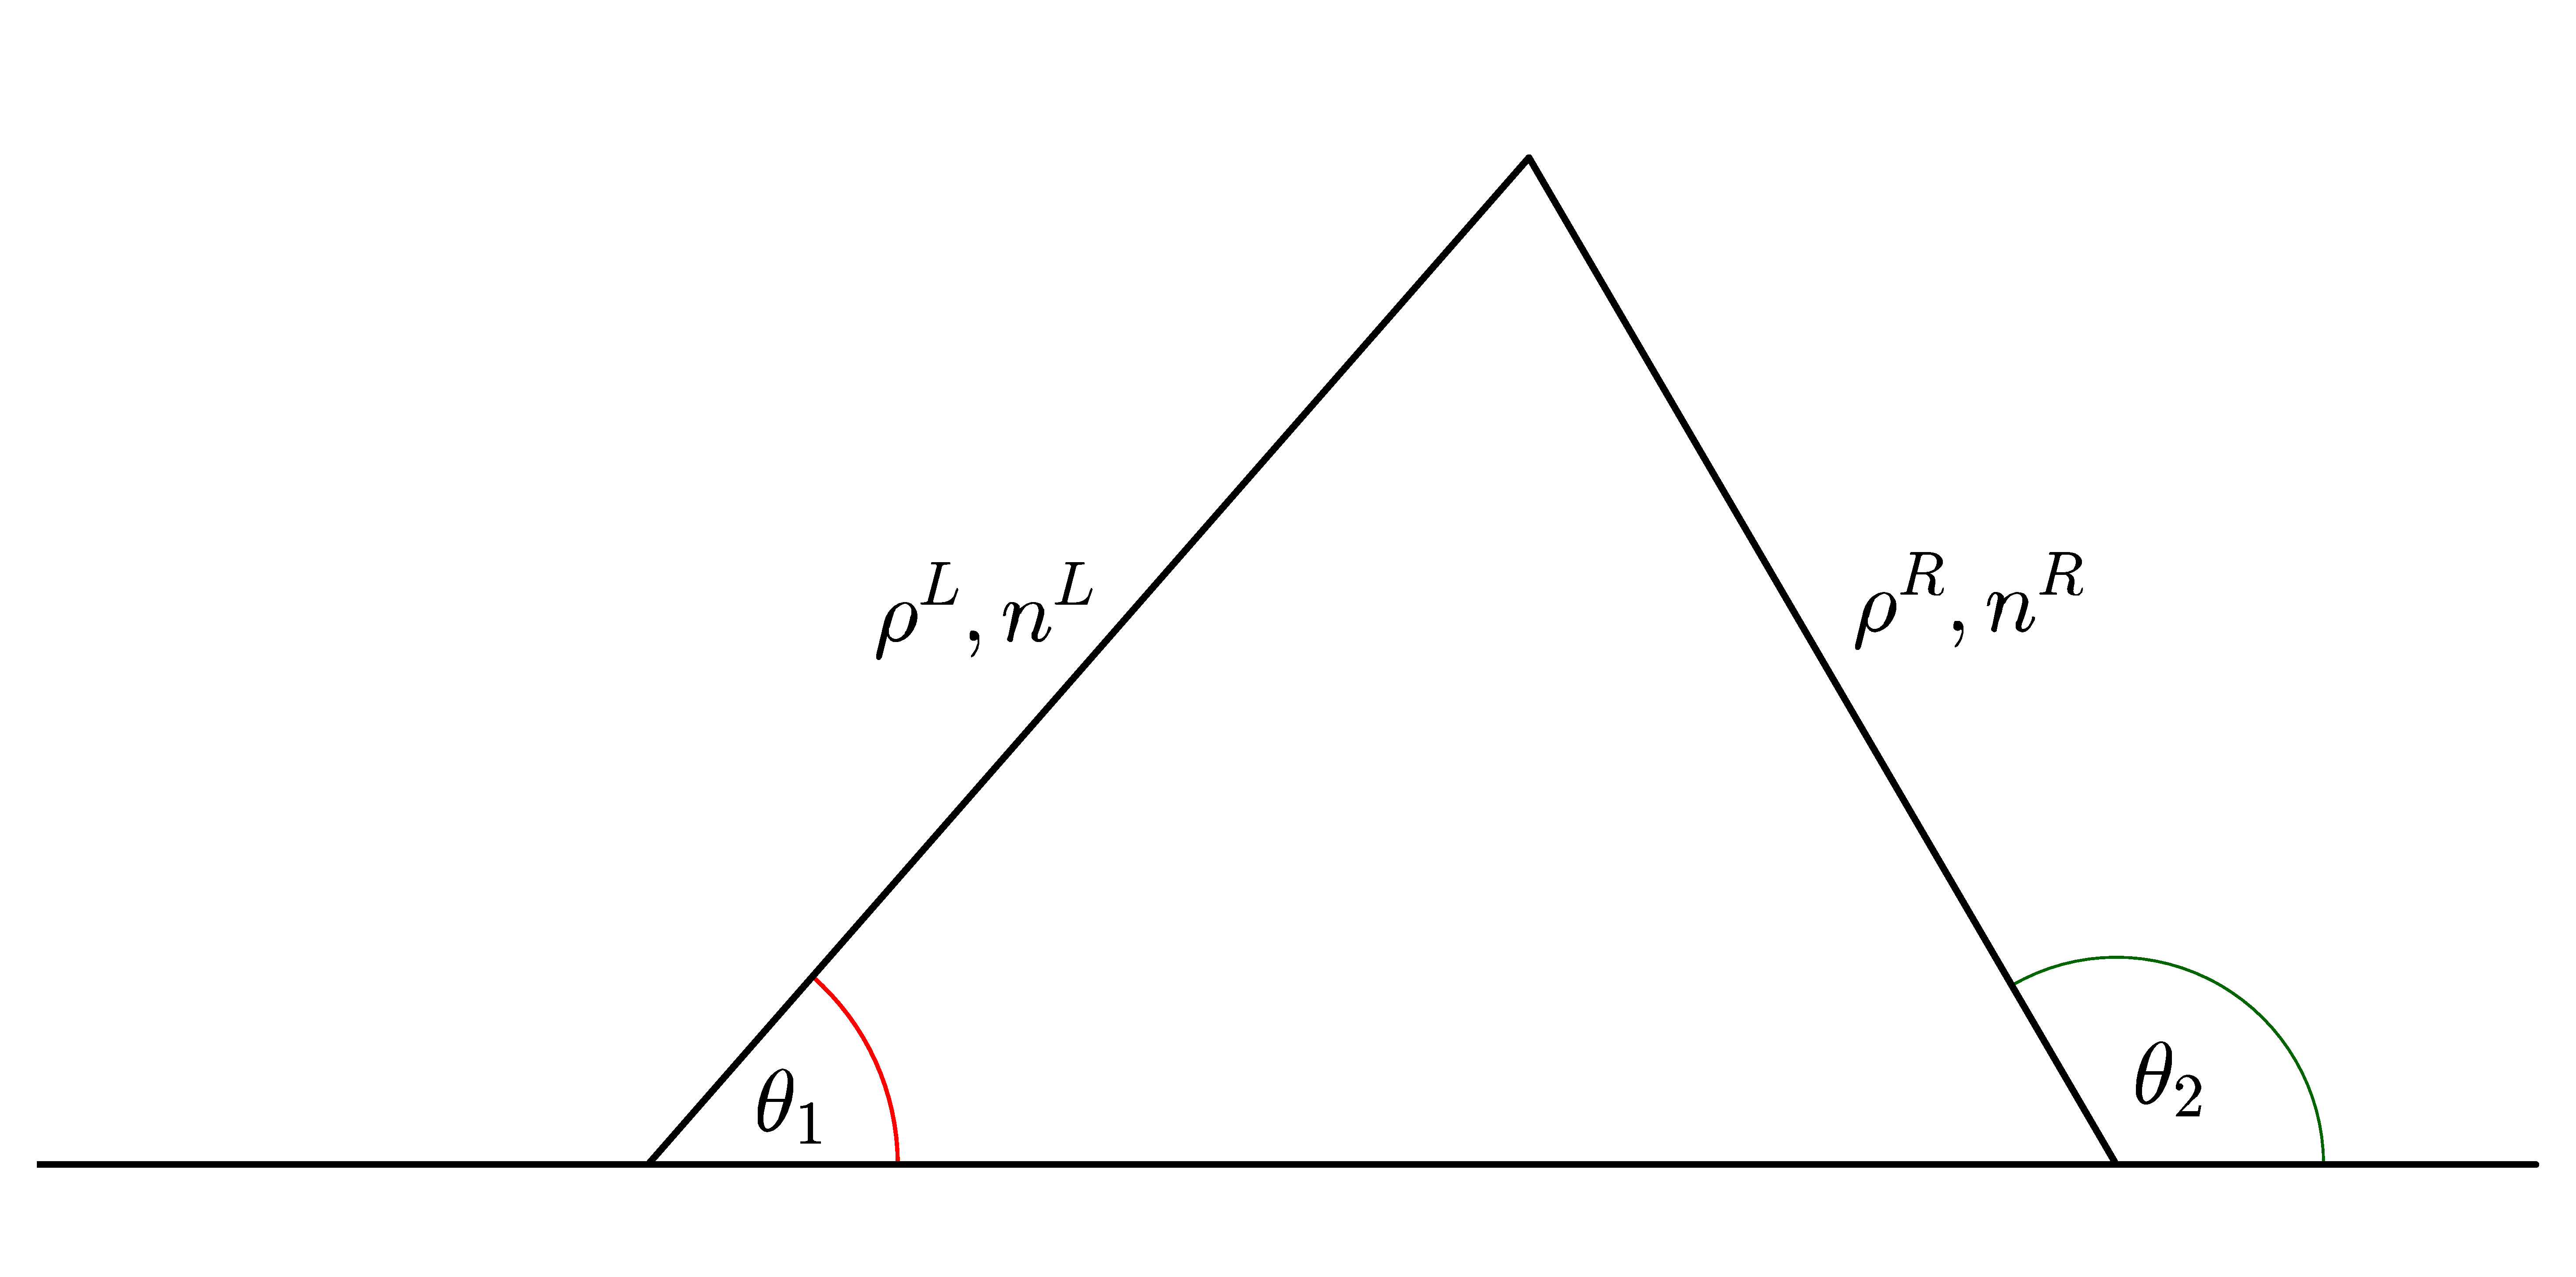
\includegraphics[width=\textwidth]{chapters/assets/dr/two-beam-line-model.png}
    \caption{Geometry of two-beam model to be used in this section. }
    \label{chap:dr-sec:two-beams-fig:two-beam-line-model}
\end{figure}



If all the beams are neutrinos, but with different energies for the left and right beams. The distribution function for beams is delta function. In fact, each beam is just half of the total neutrino number density $n_t$.

The Hamiltonian is a sum of vacuum terms, matter terms, and self-interaction terms,
\begin{equation}
   H= H_v + H_m + H_{\nu\nu}, 
\end{equation}
where
\begin{align}
   H_v =& - \eta \frac{1}{2}\omega \sigma_3 \\
   H_m =& \frac{1}{2}\lambda \sigma_3\\
   H_{\nu\nu}^L =& \frac{1}{2}\mu^R \rho^R (1-\cos(\theta_1-\theta_2))\\
   H_{\nu\nu}^R =& \frac{1}{2}\mu^L \rho^L (1-\cos(\theta_1-\theta_2)).
\end{align}
To linearize the equation of motion, we define the perturbed density matrix as
\begin{equation}
   \rho = \frac{1}{2}\begin{pmatrix}
   1 & \epsilon\\
   \epsilon^* & -1
   \end{pmatrix},
\end{equation}
where we have removed the trace part because it is alway time independent.


The linearized equation of motion becomes
\small\begin{align}
   &i \partial_z \begin{pmatrix}
   \epsilon_1 \\
   \epsilon_2
   \end{pmatrix} =  - i \begin{pmatrix}\cot\theta_1\partial_x & 0 \\
   0 & \cot\theta_2 \partial_x
   \end{pmatrix} \begin{pmatrix}
   \epsilon_1 \\
   \epsilon_2
   \end{pmatrix} \nonumber\\
   &+
   \frac{1}{2}\begin{pmatrix}
   (\lambda+ \mu_2 - \eta \omega_1 - \mu_2 \cos(\theta_1-\theta_2) )/\sin \theta_1 & -\mu_2 (1-\cos(\theta_1-\theta_2)) /\sin \theta_1\\
   -\mu_1 (1- \cos(\theta_1-\theta_2))/\sin\theta_2 & (\lambda + \mu_1 - \eta \omega_2 - \mu_1 \cos(\theta_1-\theta_2) )/\sin\theta_2
   \end{pmatrix}\begin{pmatrix}
   \epsilon_1 \\
   \epsilon_2
   \end{pmatrix},
   \label{chap:dr-sec:two-beams-eqn:line-model-two-beams-all-neutrino-linearized-eom}
\end{align}\normalsize
where
\begin{align*}
   \mu_1 =& \sqrt{2}G_F n_{t,1}\\
   \mu_2 =& \sqrt{2}G_F n_{t,2}. 
\end{align*}
   


\subsection{Left-right Symmetric Emission}


We first consider a simple case, where $\theta_1=\theta_2\equiv\theta$, $\lambda=0$, $\eta=1$, and homogeneous in $x$ direction. For simplicity we define
\begin{align*}
   \mu =& \sqrt{2}G_F (n_1 + n_2)\\
   \mu_i =& \mu \frac{n_i}{n_1+n_2}\equiv \mu f_i \\
   \xi = & 1-\cos(\theta_1-\theta_2)\\
   \omega'_i = & \lambda - \eta\omega_i.
\end{align*}

I am aware that this is not a self-consistent example since $\theta_1=\theta_2$ indicates that $\xi=0$. As we will see, no instability is present in this case. However, we keep the term $\xi$ because we need to analyze the effect of symmetry breaking. This example builds up a formalism.

The equation for perturbations becomes
\begin{equation}
   i\partial_z\begin{pmatrix}
   \epsilon_1 \\
   \epsilon_2
   \end{pmatrix} = \frac{1}{2\sin\theta} \begin{pmatrix}
   \omega'_1 + \mu f_2\xi & -\mu f_2 \xi \\
   -\mu f_1 \xi & \omega'_2 + \mu f_1 \xi
   \end{pmatrix}\begin{pmatrix}
   \epsilon_1 \\
   \epsilon_2
   \end{pmatrix}.
   \label{eqn-linearized-eom-symmetric-eg}
\end{equation}
Since $\mu$ is the most important energy scale in this problem, we scale all energies with it.
\begin{equation}
   i\partial_{\hat z}\begin{pmatrix}
   \epsilon_1 \\
   \epsilon_2
   \end{pmatrix} = \frac{1}{2\sin\theta} \begin{pmatrix}
   \hat\omega'_1 +  f_2\xi & - f_2 \xi \\
   - f_1 \xi & \hat\omega'_2 +  f_1 \xi
   \end{pmatrix}\begin{pmatrix}
   \epsilon_1 \\
   \epsilon_2
   \end{pmatrix},
\end{equation}
where
\begin{align*}
   \partial_{\hat z} =& \frac{d}{\mu dz} \\
   \hat \omega'_i =& \frac{\omega'_i}{\mu}.
\end{align*}


The characteristic equation for this equation is
\begin{equation}
   \left( ( \Omega - \hat\omega'_1 - f_2\xi )(\Omega - \hat\omega'_2-f_1\xi) - f_1 f_2 \xi^2 \right) =0,
   \label{chap:dr-sec:two-beams-eqn:two-beam-line-characteristic-eqn-simple}
\end{equation}
which is simplified to
\begin{equation*}
   (\Omega-\Omega_1)(\Omega-\Omega_2) -f_1f_2\xi^2 = 0,
\end{equation*}
where
\begin{align*}
   \Omega_1 = & \hat\omega'_1 + f_2 \xi\\
   \Omega_2 = & \hat\omega'_2 + f_1 \xi.
\end{align*}
Complete the square
\begin{equation*}
   (\Omega - (\Omega_1 + \Omega_2)/2)^2 = \frac{1}{4}(\Omega_1-\Omega_2) + f_1f_2\xi^2.
\end{equation*}
The solution becomes
\begin{equation}
   \Omega = \frac{1}{2}(\Omega_1+\Omega_2)\pm\sqrt{ (\Omega_1-\Omega_2)^2/4 + f_1f_2\xi^2 }.
\end{equation}
The condition to have positive imaginary part is
\begin{equation*}
   (\Omega_1-\Omega_2)^2 + 4f_1f_2\xi^2 < 0,
\end{equation*}
or
\begin{equation*}
   -2\sqrt{-f_1f_2\xi^2}<\Omega_1-\Omega_2<2\sqrt{-f_1f_2\xi^2},
\end{equation*}
and $f_1f_2\xi^2<0$. Recall the meaning of $f_i$,
\begin{equation*}
   f_i = \frac{n_i}{n_1+n_2}, 
\end{equation*}
instability requires that we have a spectrum crossing, i.e., $n_1$ and $n_2$ have different signs. Plug in the definitions of $\Omega_i$,
\begin{equation*}
   -2\sqrt{-f_1f_2\xi^2}< \eta(- \omega_1 + \omega_2)/\mu + (f_2 - f_1)\xi < 2\sqrt{-f_1f_2\xi^2}.
\end{equation*}
From this we can infer
\begin{itemize}
    \item $f_1f_2$ has to be negative, which means we can NOT have instabilities with only neutrinos or antineutrinos with all the symmetries we assumed. This is crossing.

\item $-\omega_1+\omega_2=0$ will remove the instability. So we have to have both neutrinos and antineutrinos.
\item $f_2-f_1$, $\eta(\omega_2-\omega_1)$, and $\mu$ set limit on each other.
\item $\theta_1=\theta_2\equiv \theta$ removes the instability since it leads to $\xi=0$. The emission has to be asymmetric in this simple two beams model. This is trivial since equal emission angle means the beams are not colliding.
\end{itemize}


% .. admonition:: But why?
%   :class: warning

%   We have these conclusions. But why?

%   What are the roles of

%   1. :math:`f_i`,
%   2. neutrino beam and antineutrino beam,
%   3. hierarchy,
%   4. neutrino number density variations,
%   5. variations of angular distributions of neutrinos,
%   6. variations of energy spectrum of neutrinos.


Another way of understanding this equation is to think of it as the growth of the length of the vector $\vec v = (\epsilon_1,\epsilon_2)^T$. For an arbitrary matrix differential equation of the form
\begin{equation*}
  \partial_z \mathbf v = \mathbf A \mathbf v,  
\end{equation*}
we can always decompose the matrix $\mathbf A$ into symmetric part and skew-symmetric part
\begin{equation*}
  \mathbf A = \frac{1}{2}(\mathbf A + \mathbf A^T) + \frac{1}{2}(\mathbf A - \mathbf A^T) \equiv \mathbf A^+ + \mathbf A^-.
\end{equation*}
We can identify the effect of $f_1-f_2$ but this is not particularly useful since we can not say anything about the eigenvalues of matrix $\mathbf A$ from the eigenvalues of matrix $\mathbf A^+$ and $\mathbf A^-$.



\subsection{Breaking Symmetries}



For a line model, the symmetries we have are
\begin{itemize}
    \item Time translation symmetry;
\item Translation symmetry along the line;
\item Energy spectrum of the beams; One of particular interest is to have different neutrino spheres for different energies which can be investigated using two beam model.
\item Number density of left and right beams;
\item Angle of left and right beams;
\item With and without matter.
\item Similar to the discussion of varying matter potential, symmetries can be broken globally, i.e., distribution as a function of spacetime coordinates.
\end{itemize}

I will discuss some of the symmetries mentioned above.



\subsubsection{Emission Angle Parity Symmetry}

The emission angles change the value of $\xi=1-\cos(\theta_1-\theta_2)$ as well as rescale the quantities by angle dependent factor $1/\sin\theta_i$.

To see the importance of angles, we can redefine some quantities
\begin{align*}
   \omega''_i=& \frac{\omega'_i}{\sin\theta_i}\\
   f''_1=&\frac{f_1}{\sin\theta_2} \\
   f''_2=&\frac{f_2}{\sin\theta_1}.
\end{align*}
The we will reach the same characteristic equation as Eqn. \ref{chap:dr-sec:two-beams-eqn:two-beam-line-characteristic-eqn-simple}. So the angles serves as shift of energy gap and angular distribution.

The region of instability changes in a convoluted way. Given angles we can always write down the expression and find out.
\begin{itemize}
    \item  The criteria of existence of instability doesn't change.
\item  The region of instability changes.
\end{itemize}


\subsubsection{Matter Effect}


Including matter will define vacuum frequencies, $\omega'_i$, which is effectively just a shift of vacuum frequencies. In the symmetric emission case, $\omega'_1-\omega'_2$ is independent of matter effect. But breaking the emission symmetry generates the degeneracy,
\begin{equation}
   \hat\omega''_1-\hat\omega''_2=( \lambda/\sin\theta_1 - \lambda/\sin\theta_2 + \eta(- \omega_1/\sin\theta_1 + \omega_2/\sin\theta_2) )/\mu`.
\end{equation}

We notice that very large matter density shift the region to very small $\mu$.

However, matter effect is not always this simple. Suppose we have different matter potential for different beams, when they collide they would have built a different phase due to matter effect.

The inhomogeneous matter effect has been studied in \cite{Mangano2014}. It can excite high Fourier moments of polarization vector, which makes a lot of sense because it generates fine structure in the x direction. This might be integrated into LESA effect.



\subsubsection{Translation Symmetry}


Translation symmetry is better explained by introducing Fourier transform in x direction. 

For each mode, a term that is proportional to Fourier mode index $m$. It only appears in diagonal elements, thus is effectively a shift of vacuum frequencies, thus energies of neutrinos.

For each Fourier mode
\begin{equation*}
   \begin{pmatrix}
   \epsilon_1 \\
   \epsilon_2
   \end{pmatrix} =  \mathbf Q(\Omega,k) e^{-i(\Omega t- k x)},
\end{equation*}
where we set $\Omega=0$.

First term in RHS of Eqn.~ \ref{chap:dr-sec:two-beams-eqn:line-model-two-beams-all-neutrino-linearized-eom} becomes
\begin{equation*}
   - i \begin{pmatrix}\cot\theta_1\partial_x & 0 \\
   0 & \cot\theta_2 \partial_x
   \end{pmatrix} \begin{pmatrix}
   \epsilon_1 \\
   \epsilon_2
   \end{pmatrix} = k \begin{pmatrix}\cot\theta_1 & 0 \\
   0 & \cot\theta_2
   \end{pmatrix} \begin{pmatrix}
   Q_1 \\
   Q_2
   \end{pmatrix}.
\end{equation*}
We now define $\hat\omega''_i$, so that
\begin{equation*}
   \hat\omega''_{k,i} = \hat \omega''_i + 2\hat k\cot\theta_i,
\end{equation*}
where $\hat k=k/\mu$.

The $k$ term contributes to the difference between $\Omega_{k,i}\equiv \hat\omega''_{k,i}+ f''_i\xi$.

We notice that instability criteria doesn't change. However, the regime of instability changes. We also know that the instability region is determined by
\begin{equation}
   \lvert \Delta\hat\omega''_{12} + 2\hat k (\cot \theta_1 - \cot\theta_2) + \Delta f''_{12}\xi \rvert < \sqrt{-f_1f_2\xi^2},
\end{equation}
where $\Delta \hat \omega''_{12} = \hat\omega''_1-\hat\omega''_2$. The instability region shift from
\begin{equation}
   -\sqrt{-f''_1f''_2\xi^2} -\Delta f''_{12}\xi < (\Delta\omega''_{12} + 2 k(\cot\theta_1-\cot\theta_2))/\mu < \sqrt{-f''_1f''_2\xi^2} -\Delta f''_{12}\xi
\end{equation}
If $\lvert \Delta\omega''_{12} + 2 k(\cot\theta_1-\cot\theta_2) \rvert$ becomes larger, the region of instability is shifted to larger $\mu$, i.e., larger number density.



\subsubsection{Number Density of Emission}


A crossing is required to have instability, i.e., $-f''_1f''_2>0$. Meanwhile the number density on the left and right have little effects on the existance of instability. It shifts the region of instability for $\mu$.


\subsubsection{Energy of Emission}



Different energy of two beams will make sure $-\omega_1 + \omega_2\neq 0$. It has no effects on the criteria but changes the $\mu$ region of instability.


% \subsubsection{Time Translation Symmetry}



% .. admonition:: Time Translational Symmetry
%   :class: warning

%   How about time translational symmetry? I need to write down the equation of motion that is related to time.

%   Two limits are of particular interest.

%   1. Adiabatic limit,
%   2. Superfast time variants.




\subsubsection{General Solutions to Line Model}


For completeness, we solve the general line model, c.f.~Eqn.~\ref{chap:dr-sec:two-beams-eqn:line-model-two-beams-all-neutrino-linearized-eom}. We know that real symmetric matrix has only real eigenvalues, from which we infer that $\mu_1=\mu_2$ and $\theta_1=\theta_2$ removes the instability.
For translation symmetric models, that is $\partial_x\to 0$, we have the eigenvalues
\begin{equation*}
   \Omega = \frac{1}{4}(A\pm B),
\end{equation*}
where
\begin{align*}
   A=& -\eta \omega_1/\sin\theta_1 - \mu_2 /\sin\theta_1 + \eta \omega_2 /\sin\theta_2 + \mu_1 \xi /\sin\theta_2 + \lambda(1/\sin\theta_1 + 1/\sin\theta_2)  \\
   B=& \left(
      -4[(\lambda-\eta\omega_1)(\lambda +\eta\omega_2) + (\lambda (\mu_1-\mu_2) -\eta (\mu_1\omega_1 + \mu_2\omega_2) )\xi ] \sin\theta_1 \sin\theta_2\right. \\
      &\left.+ [(\lambda + \eta\omega_2 + \mu_1\xi) \sin\theta_1 + (\lambda - \eta \omega_1 - \mu_2\xi) \sin\theta_2 ]^2
   \right)^{1/2}/(\sin\theta_1\sin\theta_2)\\
   \xi=&1-\cos(\theta_1-\theta_2).
\end{align*}


For antineutrinos, I only need to change $\mu_i\to -\bar\mu_i$ and $\omega_i\to -\bar\omega_i$, where $\bar\mu=\sqrt{2}G_F \bar n_t$, so that the equation becomes
\small\begin{align*}
  &i \partial_z \begin{pmatrix}
  \epsilon_1 \\
  \epsilon_2
  \end{pmatrix} =  - i \begin{pmatrix}\cot\theta_1\partial_x & 0 \\
  0 & \cot\theta_2 \partial_x
  \end{pmatrix} \begin{pmatrix}
  \epsilon_1 \\
  \epsilon_2
  \end{pmatrix} \\
  &+
  \frac{1}{2}\begin{pmatrix}
  (\lambda-\bar\mu_2 + \eta \bar\omega_1 + \bar\mu_2 \cos(\theta_1-\theta_2) )/\sin \theta_1 & \bar\mu_2 (1-\cos(\theta_1-\theta_2)) /\sin \theta_1 \\
  \bar\mu_1 (1- \cos(\theta_1-\theta_2))/\sin\theta_2 & (\lambda -\bar\mu_1 + \eta \bar\omega_2 +\bar\mu_1 \cos(\theta_1-\theta_2) )/\sin\theta_2
  \end{pmatrix}\begin{pmatrix}
  \epsilon_1 \\
  \epsilon_2
  \end{pmatrix}
\end{align*}\normalsize

Assume that the left beam is neutrino beam and the right beam is antineutrno beam. The linearized equation of motion becomes
\small
\begin{align*}
  &i\partial_z \begin{pmatrix}
  \epsilon_1 \\
  \epsilon_2
  \end{pmatrix} =  -i\begin{pmatrix}
  \cot\theta_1 \partial_x & 0 \\
  0 & \cot\theta_2 \partial_x
  \end{pmatrix}\begin{pmatrix}
  \epsilon_1 \\
  \epsilon_2
  \end{pmatrix} \\
  &+ \frac{1}{2}\begin{pmatrix}
  (\lambda - \bar\mu - 2\eta \omega_1 + \bar\mu \cos(\theta_1-\theta_2) )/\sin\theta_1 & \bar\mu (1-\cos(\theta_1-\theta_2))/\sin\theta_1 \\
  -\mu(1-\cos(\theta_1-\theta_2))/\sin\theta_2 & (\lambda + \mu + \eta \omega_2 - \mu \cos(\theta_1-\theta_2) )/\sin\theta_2
  \end{pmatrix}\begin{pmatrix}
  \epsilon_1 \\
  \epsilon_2
  \end{pmatrix}
\end{align*}
\normalsize


% Numerical Calculations
% ~~~~~~~~~~~~~~~~~~~~~~~~~~~~~~


% We assume the two beams have different energy, as indicated by :math:`\omega_1` and :math:`\omega_2` in Eq. \ref{chap:dr-sec:two-beams-eqn:line-model-two-beams-all-neutrino-linearized-eom}


% For numerical calcualtions, we scale quantities using :math:`\mu`.

% With symmetric angles for the two beams, I didn't find instabilities. However, :math:`\theta_1\neq \theta_2` leads to instabilities in IH, which is consistant with our expections.



% For NH:


% .. image:: assets/some-clarifications/allneutrinos/line-two-beam-eta-1-lambda-0-mu-10-alpha-0.5-theta1-pi-div-3-theta2-pi-div-6.png
%   :width: 31%
% .. image:: assets/some-clarifications/allneutrinos/line-two-beam-eta-1-lambda-0-mu-10-alpha-1.-theta1-pi-div-3-theta2-pi-div-6.png
%   :width: 31%
% .. image:: assets/some-clarifications/allneutrinos/line-two-beam-eta-1-lambda-0-mu-10-alpha-1.5-theta1-pi-div-3-theta2-pi-div-6.png
%   :width: 31%

% .. image:: assets/some-clarifications/allneutrinos/line-two-beam-eta-1-lambda-0-mu-10-alpha-0.5-theta1-pi-div-6-theta2-pi-div-3.png
%   :width: 31%
% .. image:: assets/some-clarifications/allneutrinos/line-two-beam-eta-1-lambda-0-mu-10-alpha-1.-theta1-pi-div-6-theta2-pi-div-3.png
%   :width: 31%
% .. image:: assets/some-clarifications/allneutrinos/line-two-beam-eta-1-lambda-0-mu-10-alpha-1.5-theta1-pi-div-6-theta2-pi-div-3.png
%   :width: 31%

% .. image:: assets/some-clarifications/allneutrinos/line-two-beam-eta-1-lambda-0-mu-10-alpha-0.5-theta1-pi-div-3-theta2-pi-div-3.png
%   :width: 31%
% .. image:: assets/some-clarifications/allneutrinos/line-two-beam-eta-1-lambda-0-mu-10-alpha-1.-theta1-pi-div-3-theta2-pi-div-3.png
%   :width: 31%
% .. image:: assets/some-clarifications/allneutrinos/line-two-beam-eta-1-lambda-0-mu-10-alpha-1.5-theta1-pi-div-3-theta2-pi-div-3.png
%   :width: 31%



% Non-local Symmetry Breaking
% -----------------------------









\section{\label{chap:dr-sec:fast-mode}Fast Mode}


In a paper by Chakraborty et al~\cite{Chakraborty2016}, they showed that neutrino flavor instabilities can grow with a rate that is proportional to the neutrino density, which has much faster oscillation frequencies than vacuum oscillations. For such a fast growth to happen, the author considered head on colliding neutrino beams. The derivation is much similar to what has been shown in the previous section.

As an estimation, the frequencies of vacuum oscillation is
\begin{align*}
   \omega_{\mathrm v} =& \frac{\Delta m^2}{2E} \\ \sim& 6.3\times 10^{-3} \mathrm{m}^{-1}  \frac{\Delta m^2_{32}}{2.5\times 10^{-3} \mathrm{eV}^2 } \frac{1MeV}{E} \\
   \sim & 1.90\times 10^{-4}  \mathrm{m}^{-1}  \frac{\delta m^2}{7.5\times 10^{-5}\mathrm{eV}^2} \frac{1\mathrm{MeV}}{E},
\end{align*}
where $E$ is the neutrino energy. The corresponding oscillation wavelength is simply give by
\begin{align*}
   \lambda_{12} = & 2\pi/\omega_{12} \sim 1 \mathrm{km}\\
   \lambda_{32} = & 2\pi/\omega_{32} \sim 33.1 \mathrm{km}.
\end{align*}
The fast modes instability grows with a rate proportional to the neutrino potential $\mu=\sqrt{2}G_F n_\nu$, which is very large in dense neutrino media. A large growth rate indicates a faster flavor transformation than vacuum oscillations.




% \subsection{\label{chap:dr-sec:fast-mode-subsec:introduction}Introduction}

% (Should talk about some very very basic backgrounds like the applications and why it is important.)





\subsection{\label{chap:dr-sec:fast-mode-subsec:dr}Dispersion Relation of Neutrino Flavor Conversion}

We consider two-flavor scenario ($\nu_{\mathrm e}$ and $\nu_{\mathrm x}$) of neutrino oscillations. We also assume that all neutrinos and antineutrinos are emitted as electron flavor. The flavor evolution of neutrino ensemble depends on flavor density matrices of neutrinos $\rho$ and antineutrinos $\bar\rho$ with energy $E$, direction of velocity $\hat{\mathbf v}$,
\begin{equation}
\ii (\partial_t + \mathbf v\cdot \mathbf{\nabla}) \rho = \left[H, \rho_n \right],
\label{eqn-liouville-eqn}
\end{equation}
where $H$ is the Hamiltonian for neutrino oscillations. In the context, Hamiltonian depends on three different contributions from vacuum oscillations $H_{\mathrm v}$, interactions with matter $H_{\mathrm m}$, and interactions with neutrinos themselves $H_{\nu\nu}$. In this work, we ignore vacuum and matter terms since the concentration is on fast neutrino oscillations, which would occur even without neutrino mass differences \cite{Chakraborty2016,Dasgupta2017}. In order to calculate the neutrino self-interaction term $H_{\nu\nu}$, the distribution of neutrinos (antineutrinos) $f_{\nu_{\mathrm e}(\bar \nu_{\mathrm e})}(\hat{\mathbf v}, E)$ and $f_{\nu_{\mathrm x}(\bar \nu_{\mathrm x})}(\hat{\mathbf v}, E)$ is required, where $E$ is the energy of neutrinos (antineutrinos). We have
\begin{equation}
H_{\nu\nu} = \sqrt{2} G_{\mathrm F} \iint \frac{\mathrm d \cos\theta' \mathrm d\phi'}{4\pi} v^\mu v'_\mu \int \frac{E'^2 \mathrm d E'}{2\pi^2} \left( (f_{\nu_{\mathrm e}}' - f_{\nu_{\mathrm x}}' )\rho' -  (f_{\bar\nu_{\mathrm e}}' - f_{\bar\nu_{\mathrm x}}' ) \bar\rho' \right),
\end{equation}
where $v^\mu = ( 1, \sin\theta\cos\phi, \sin\theta\sin\phi, \cos\theta )^{\mathrm T}$ is the four velocity of (anti)neutrinos in our spherical coordinate system. Without vacuum contribution, the equation of motion for antineutrinos has the same form \cite{Duan2010}.

We follow the same assumption in reference \cite{Izaguirre2016a} that the the distribution of $\nu_x$ and $\bar\nu_x$ are the same, namely $ f_{\nu_{\mathrm x}}(\hat{\mathbf v},E)  - f_{\bar\nu_{\mathrm x}}(\hat{\mathbf v},E)=0$. In addition, we have the same definition of electron lepton number (ELN) of neutrinos travelling in direction $\hat{\mathbf v}$ \cite{Izaguirre2016a},
\begin{equation}
G(\hat{\mathbf v}) =  \sqrt{2}G_{\mathrm F} \int \frac{E'^2 \mathrm d E'}{2\pi^2} ( f_{\nu_{\mathrm e}}(\cos\theta',\phi',E')  - f_{\bar\nu_{\mathrm e}}(\cos\theta',\phi',E')  ).
\end{equation}
To perform linear stability analysis, we assume that the density matrix has the form
\begin{equation}
\rho = \bar \rho = \begin{pmatrix}
1 & \epsilon \\
\epsilon^* & 0
\end{pmatrix},
\end{equation}
where $\lvert \epsilon \rvert \ll 1$. As a result, the linearized equations of motion depends only on $G(\hat{\mathbf v})$ and $\hat{\mathbf v}$. We also assume that all neutrinos and antineutrinos undergo the same behavior in linear regime, $\epsilon = \tilde\epsilon e^{-\ii (\Omega t - \mathbf K\cdot \mathbf x)}$. Izaguirre, Raffelt, and Tamborra defined the polarization tensor \cite{Izaguirre2016a},
\begin{equation}
\Pi^\mu_{\phantom{\mu}\nu} = 1 + \int \frac{d\Omega}{4\pi} G(\theta,\phi) \frac{v^\mu v_\nu}{\omega- k \hat{\mathbf k}\cdot \hat{\mathbf v} },
\end{equation}
which defines the dispersion relation $\Pi^\mu_{\phantom{\mu}\nu} a^\nu = 0$, with $a^\nu = \int \frac{d\cos\theta' d\phi'}{4\pi} G(\hat{\mathbf v}') v^\nu \tilde\epsilon$. We find the nontrivial solutions by setting \cite{Izaguirre2016a},
\begin{equation}
\operatorname{det}\left( \Pi^\mu_{\phantom{\mu}\nu} \right) = 0.
\label{eqn-dr-determinant-equation}
\end{equation}


For simplicity, we consider axial symmetric neutrino emission so that Eq. \eqref{eqn-dr-determinant-equation} becomes
\begin{align}
&\det \left( \omega \mathrm{I} + \frac{1}{2}
\begin{pmatrix}
   I_0 & 0 & 0 & -I_1 \\
   0 & -\frac{1}{2} (I_0 - I_2) & 0 & 0 \\
   0 & 0 & -\frac{1}{2} (I_0 - I_2) & 0 \\
   I_1 & 0 & 0 & -I_2
\end{pmatrix}\right) \nonumber\\
&=0,
\label{eqn-det-polarization-tensor-axial}
\end{align}
where $\mathbf I$ is the rank 4 identity matrix and
\begin{equation}
   I_m =\int_{-1}^{1} d u G(u) \frac{u^m}{1 -  \left(\lvert k\rvert /\omega\right) u }.
\end{equation}
where we define $u=\cos\theta$. Eq. \eqref{eqn-det-polarization-tensor-axial} is equivalent to the result in reference \cite{Raffelt2013}. $\lvert k \rvert /\omega$ is defined as the refractive index $n$ of the flavor wave. For spectrum $G(u)$ without zero values, the forbidden region is given by $1 -  \left(\lvert k\rvert /\omega\right) u\leq 0$.

The dispersion relations can be categorized into two different types by symmetries. To incorporate azimuthal symmetry, we define solutions related to the first and second element of $a^\nu$ ($\nu=1,2$) to be multi-azimuthal angle (MAA) solutions since they are the only solutions that depend on azimuthal angle $\phi$. The other solutions which are related to $\nu=0,3$ are defined to be the multi-zenith angle (MZA) solutions. The MAA solution is related to symmetry breaking in azimuthal angle only, which is determined by
\begin{equation}
   \omega = \frac{1}{4}(I_0 - I_2).
   \label{eqn-maa}
\end{equation}
Similarly, the MZA solution is related to symmetry breaking in both azimuthal angle and zenith angle, which is
\begin{equation}
\omega = - \frac{1}{4} \left( I_0 - I_2 \pm \sqrt{ (I_0 + I_2 - 2 I_1) (I_0 + I_2 + 2 I_1) } \right).
\label{eqn-mza}
\end{equation}
We denote the solution associated with $+$ sign in Eq. \eqref{eqn-mza} as MZA+, while the solution assocated with $-$ sign as MZA-. The two solutions are connected to each other in dispersion relations. In general, it doesn't provide physical insights to distingush the two branches of solutions since they are simply two branches of the solution.

The solutions to Eq. \eqref{eqn-maa} and Eq. \eqref{eqn-mza} are dispersion relations $D(\omega,\mathbf k)$ for a chosen direction of $\hat{\mathbf k} = \hat{\mathbf z}$ with axial symmetric neutrino emission.



%%%%%%%%%%%%%%%%%
%% To BE Added
%%%%%%%%%%%%%%%%
% {\color{red}{\bf HAVE TO EXPLAIN THE IDEA OF GAP AND INSTABILITY HERE. Maybe Later?}}






\subsection{\label{chap:dr-sec:fast-mode-subsec:instabilities-and-gaps}Instabilities and Gaps}

In reference \cite{Izaguirre2016a}, the authors relate gaps in dispersion relation to instabilities of neutrino oscillations. In this section, we review the idea of correspondence between gaps and instabilities first. Then we show that this relation is not a solid theory that can be generalized to all cases.

We continue the discussion of axial symmetric neutrino emissions but with discretized zenith angles $\theta$ thus discretized $u$. Hence the ELN is independent of azimuth angle $\phi$. For neutrino emission with $2$ zenith angles, the ELN spectrum is
\begin{equation}
G(u)= \sum_{i=1}^2 g_i \delta(u - u_i).
\end{equation}

The MAA solution becomes an equation of hypobola for $\omega$ and $k$, which has asymptotes $\omega = k u_i$ for $i=1,2$. Meanwhile, hyperbola equation has two solutions of $\omega$ ($k$) for any given real $k$ ($\omega$). The solutions are either real which indicates stable solutions or complex which indicates exponential growth or decrease in linear regime. On the other hand, non-existence of real solutions of $\omega$ ($k$) for given real $k$ ($\omega$) is equivalent to gap in dispersion relation. Thus the equivalence of gap and instabilities is guaranteed in neutrino emission with two-zenith-angle emission. The numerical calculations is normalized using the maximium value in spectrum which is a convention we follow for all discrete emission calculations. Unit for $\omega$ and $k$ can be determined once the exact spectrum is determined. Upper panels of Fig. \ref{fig-dr-db} is reproduction of left panels of Fig. 1 in reference \cite{Izaguirre2016a}. The dispersion relation is shown as black lines. The real part $\omega_{\mathrm R}$ is shown as red solid lines. $\omega_{\mathrm R} \pm \omega_{\mathrm I}$ are shown are red dashed lines, where $\omega_{\mathrm I}$ is the imaginary part of $\omega$.



\begin{figure}[!htb]
\minipage{0.49\textwidth}
  \includegraphics[width=\linewidth]{chapters/assets/dr/spectDBWC1DRDBMAAPltBlob.pdf}
\endminipage\hfill
\minipage{0.49\textwidth}
  \includegraphics[width=\linewidth]{chapters/assets/dr/spectDBWC1DRDBMZAPltBlob.pdf}
\endminipage\hfill
\newline
\minipage{0.49\textwidth}
  \includegraphics[width=\linewidth]{chapters/assets/dr/spectDB3WC4DRDBMAAPltBlob.pdf}
\endminipage\hfill
\minipage{0.49\textwidth}
  \includegraphics[width=\linewidth]{chapters/assets/dr/spectDB3WC4DRDBMZAPltBlob.pdf}
\endminipage\hfill
\caption{Dispersion relation and instabilities of two zenith angles spectrum (upper panels) and three zenith angles spectrum (lower panels). The black lines are the dispersion relations and the colored dots are examples of complex $\omega$ for real $k$. The left panels are the dispersion relation and linear stability analysis of MAA solutions while the right panels are for MZA solutions.}
\label{fig-dr-db}
\end{figure}



In core collapse supernova and neutron star mergers, neutrino emission is not in discrete zenith angles. More realistic models involve continuous zenith angle ELN spectra. In the case that the smooth and continuous ELN spectrum has no crossing, gap indeed indicates instabilities, as shown in reference \cite{Izaguirre2016a}. In this section we prove that the instabilities in MAA, MZA+, or MZA- solution can only appear in either region $\omega\leq 0$ or region $\omega \geq 0$. As it suggests, the instability regions propagate only between the dispersion relation curves and the axis $\omega=0$. We reproduced the calculation in reference \cite{Izaguirre2016a} using the same Garching core-collapse supernova data set \cite{garching-ccsn-data}. The spectrum shown in the left panel of Fig. \ref{fig-garching} is polynomial fitting of the Garching 1D supernova simulation data. On the right of Fig. \ref{fig-garching}, the dispersion relation for MAA (MZA) solution is shown as red (green, blue) solid lines. Instabilities associated with MAA (MZA) solution is shown as light red (light green, light blue) blobs. The two branches of MZA solutions appear at the top half (MZA+) and lower half (MZA-). The result shows that instabilities occur either in region $\omega>0$ or region $\omega<0$ and with limits set the dispersion relation. We will prove that the instabilities appear between the dispersion relation and the axis $\omega=0$.






\begin{figure}
   \minipage{0.49\textwidth}
     \includegraphics[width=\linewidth]{chapters/assets/dr/spectGarchingPlt.pdf}
   \endminipage\hfill
   \minipage{0.49\textwidth}
   \includegraphics[width=\linewidth]{chapters/assets/dr/spectGarchingDRLSAPltBlob.pdf}
   \endminipage\hfill
   \caption{Dispersion relation and linear stability analysis (right panel) for a spectrum constructed from Garching 1D simulation data (left panel). Solid red line is dispersion relation for MAA solution while blue and green lines are for MZA solutions. Light red (green and green) blob is instability for MAA (MZA) solution.
    }
   \label{fig-garching}
\end{figure}




% \subsection{\label{sec-omega-to-zero}Instabilities at $\omega\to 0$}

Suppose we are looking for complex solutions for given real omega as in Fig. \ref{fig-garching}, MAA solution Eq. \eqref{eqn-maa} is rewritten as a function $k(\omega/k)$. More explicitly, we have to solve the integral function to find out $k$ for real $\omega$,
\begin{equation}
   k = \frac{1}{4} \int \mathrm du G(u) \frac{ 1 - u^2 }{ \omega/k - u }.
   \label{eqn-k-omega-relation}
\end{equation}
To investigate how instabilities developed around the horizental axies, we solve Eq. \eqref{eqn-k-omega-relation} in the limit $\omega\to 0$. For complex $k$, the integral can be decomposed into the principal value $\operatorname{Re}(k)$ and imaginary part $\operatorname{Im}(k)$ using Sokhotski–Plemelj theorem,
\begin{subequations}
\begin{align}
\operatorname{Re}(k) =& \frac{1}{4}\left(  \mathcal{P} \int \mathrm d u G(u) \frac{ 1 - u^2 }{ - u }  \right)\label{eqn-re-k-arbitrary-spectrum} \\
\operatorname{Im}(k) =&  \frac{\pi}{4}G(0) \operatorname{Sign}\left( \omega \right) \operatorname{Sign}\left(  \operatorname{Im}(k)  \right).
\label{eqn-im-k-arbitrary-spectrum}
\end{align}
\end{subequations}
Assuming no crossing is found in sepctrum $G(u)$ at $u=0$, Eq. \eqref{eqn-im-k-arbitrary-spectrum} shows that $\omega$ must have the same sign as $G(0)$ if we find nonzero imaginary part in $k$. We conclude that instabilities can only grow either in the upper plane $\omega>0$ or lower plane $\omega<0$. What's more, the value of $k$ at limit $\omega\to 0$ can be solved out of Eq. \eqref{eqn-re-k-arbitrary-spectrum} and Eq. \eqref{eqn-im-k-arbitrary-spectrum}. For instabilities the imaginary part of $k$ tells us the growth rate is,
\begin{equation}
   \lvert \operatorname{Im}(k) \rvert  =  \frac{\pi}{4}\lvert G(0)\rvert .
\end{equation}
Similar result is obtained for MZA solutions,
\begin{align}
&\left(4\operatorname{Re}(k) - \mathcal P \int \frac{G(u)}{u} \mathrm d u + U_1 \right)^2  - \left( \operatorname{Sign}(\omega \operatorname{Im}(k) )\pi G(0) +4 \operatorname{Im}(k) \right)^2 \\
% =&\left( \mathcal P \int \frac{G(u)}{u} \mathrm d u + U_1 \right)^2 -1 - 4 U_0^2  \\
% &\left( 4 \operatorname{Re}(k) - \mathcal P \int \frac{G(u)}{u} \mathrm d u + U_1 \right) \left( \pi \operatorname{Sign}(\omega \operatorname{Im}(k) ) G(0) + 4 \operatorname{Im}(k) \right) \\
=& - \left( \mathcal P \int \frac{G(u)}{u} \mathrm du + U_1 \right) \pi \operatorname{Sign}(\omega \operatorname{Im}(k) ) G(0),
\end{align}
where $U_m = \int G(u) u^m \mathrm du$ and all the integrals are over all the sepctrum. The equations are quadratic in both $\operatorname{Re}(k)$ and $\operatorname{Im}(k)$ so the real solutions can be calculated and verified with linear stability analysis. The imaginary part $\operatorname{Im}(k)$
\begin{equation}
   \operatorname{Im}(k) = - \frac{1}{4} \pi G(0) \operatorname{Sign}(\omega \operatorname{Im}(k) ) \left(  1 \pm \frac{ \mathscr P \int \frac{G(u)}{u} du + \int G(u) u du }{ 4 \operatorname{Re}(k) - \mathscr P \int \frac{G(u)}{u} du + \int G(u) u du }  \right)
\end{equation}
determines that the two different solutions are either in the region $\omega>0$ or in the region $\omega<0$ which corresponds to MZA+ and MZA- solutions. The instabilities in the two regions are not continuous at $\omega=0$.



\subsection{\label{chap:dr-sec:fast-mode-subsec:instability-to-gap}Instabilities Do Not Always Show Up as Gap}

Even though the concept of gap leads to instabilities works well for the models in \ref{chap:dr-sec:fast-mode-subsec:instabilities-and-gaps}, it can not be generalized to arbitrary number of emission angles nor to continuous spectra with crossings. As an example, we perform linear stability analysis of the three zenith angles emission configuration which is determined by a cubic function both in $\omega$ and $k$. Three solutions of $k(\omega)$ for given real $\omega(k)$  are expected. As long as real solutions disappear, complex solutions emerge, which leads to instabilities occur even without an actual gap. Rather the decrease in the number of real solutions for fixed $\omega$ or $k$ corresponds to the instabilities. As an example, we plotted dispersion relation and instabilities for three zenith angles in lower panels of Fig. \ref{fig-dr-db}. For a given value of $\omega$ such as $\omega= 0.5$, the three MAA solutions (Fig. \ref{fig-dr-db} lower left panel) of $k$ are $k=-4.6, 0.29, 1.2$. All three solutions are all real and indicate no spatial instabilities which is confirmed by calculation of instabilities shown as red blob. However, for another real $\omega = 0.2$, we find only one real solution $k=0.4$ from dispersion relation. The other solutions are complex and proven to be $k = -0.557106\pm 0.966535\mathrm i$ where the value with positive imaginary part leads to exponential growth. We conclude that instabilities doesn't require gap in dispersion relation except for two emission angles.


We will prove that instabilities for continuous emission angles do not necessarily correspond to gap in dispersion relation. In the earlier works of fast modes, Sawyer analyzed a box shaped angular distribution of neutrino emission \cite{Sawyer2016}. To address the generality of our conclusion, we repeat the calculation for box spectrum with crossing.

We construct a box spectrum with value $-0.1$ within $u\in [-1,-0.3)$ and value $1$ within $[-0.3,1]$ as shown in the top left panel of Fig. \ref{fig-box-c1}. As in the discrete emission case, we normalize all quantities using the maximium value of the spectrum. With the spectrum defined, we calculate the dispersion relation and find out complex values of $k$ for real $\omega$. The result shows that the dispersion relation of both MAA solution and MZA solution contains only one curve. No gap is formed but we observe instabilities between this curve and $\omega=0$ in MAA solution as well as two unstable regions of $k$ in MZA solution, which are plotted as red lines.


\begin{figure}
   % \minipage{0.49\textwidth}
   %   \includegraphics[width=\linewidth]{chapters/assets/dr/spectBoxC1Spectrum.pdf}
   % \endminipage\hfill
   \minipage{0.49\textwidth}
   \includegraphics[width=\linewidth]{chapters/assets/dr/spectBoxC1MAADRPltBlob.pdf}
   \endminipage\hfill
   \minipage{0.49\textwidth}
   \includegraphics[width=\linewidth]{chapters/assets/dr/spectBoxC1MZADRPltBlob.pdf}
   \endminipage\hfill
   \caption{Dispersion relation and linear stability analysis for box spectrum. The box spectrum is defined to be $-0.1$ within range $u\in [-1,-0.3)$ and $1$ within range $u\in [-0.3,1]$. Left panel shows the dispersion relation and the complex $k$ for real $\omega$ for MAA solution. Right panel is the corresponding result for MZA solution. Dash-dotted gray lines are $\omega= \pm k$ which sets the boundaries of the forbidden region for dispersion relation.
    }
   \label{fig-box-c1}
\end{figure}





\section{\label{chap:dr-sec:conclusion}Conclusion}


We have reviewed that dispersion relation gap and instabilities are the same thing for neutrino emission with two zenith angles for the quadratic nature of the problem. As for more realistic spectrum, we have proved that instabilities propagate in regions of either $\omega>0$ or $\omega<0$ and never cross $\omega=0$. Hence the dispersion relation gaps should be defined as gaps between the dispersion relation curves and the axis $\omega=0$ instead of the dispersion relation curves. We have also showed that instabilities is not necessarily shown as gap in dispersion relations for neutrino emission with more than two zenith angles and box spectrum with crossing. Through the discussions, we demonstrated that the relation between dispersion relation gaps and instabilities should be used with caution.


% %!TEX root = ../dissertation.tex


\chapter{\label{chap:halo}Neutrino Halo Problem}


One of the big questions about neutrino oscillations in supernovae is the so called halo problem. Cherry et al showed that neutrino flavor conversions are greatly affected by the back scattered neutrinos in supernovae~\cite{Cherry2012}. Neutrinos around supernovae are scattered and some of them are scattered to move almost backward. On the other hand, neutrino self-interactions is proportional to the inner product of momenta of neutrinos, which leads to the dependence on $1-\cos\theta$ where $\theta$ is the angles between momenta of two neutrinos. Most of the research has been concentrating on mostly forward scattering, with small values for $1-\cos\theta$. For back ward scattered neutrinos, the interaction potential can be much larger than the forward scattered neutrino contributions. Though the work by Sarikas et al showed that matter suppression is still significant within this region~\cite{Sarikas2012a}, it is not clear how exactly the neutrino halo alters neutrino oscillations. The halo problem itself is worth more calculations.


\section{\label{chap:halo-sec:line}Line Model}

We continue to use the simplified line model and build our intuitions out of it. The halo problem is simplified to have neutrinos emitted from a line $z=0$ homogeneously, which are reflected from a certain distance $z=L$. In principle, the reflection angles doesn’t have to be Snell’s law. The scattering can be in any angle with different amplitudes. Here I am using this very simple Snell’s law just to explore the effect of halo. It's crucial to keep an eye on the simplifications in this line model.
\begin{itemize}
    \item Neutrinos are emitted from a line, which is not the case in a real supernova.
    \item Neutrinos are emitted with translation symmetry on the line. Breaking the symmetry might bring in other qualitatively different results.
    \item Neutrinos are reflected from a certain surface $z=L$, which is different from reality where neutrinos are scattered everywhere.
    \item Neutrinos are reflected according to Snell's law.
    \item Neutrinos are homogeneously reflected at $z=L$.
\end{itemize}



\begin{figure}
    \centering
    \includegraphics[width=\textwidth]{chapters/assets/halo/line-model.pdf}
    \caption{Line model used for halo problem. Neutrinos are emitted from the bottom line and reflected at the top line.}
    \label{chap:halo-sec:line-fig:line-model}
\end{figure}


The algorithm that I used is relaxation method. The algorithm is meant to find the equilibrium state of neutrino oscillations with the presence of halo.
\begin{enumerate}
\item Calculate forward beam using 0 backward beam;
\item Calculate backward beam using forward beam calculated in 1;
\item Calculate forward beam using backward beam calculated in 2;
\item Repeat until the beams reach equilibrium.
\end{enumerate}


\section{\label{chap:halo-sec:line-sym}Neutrino Beams Only}

As a first step, I calculated neutrino oscillations with only neutrino beams. Before we rush to the numerical results, I linearized the equation of motion and worked out the linear stability analysis.

In linear regime, we define the density matrices for forward and backward beams to be
\begin{align*}
   \rho_F &= \frac{1}{2} \begin{pmatrix}
   1 & \epsilon_F \\
   \epsilon_B^* & -1
   \end{pmatrix} \\
   \rho_B &= \frac{1}{2} \begin{pmatrix}
   1 & \epsilon_B \\
   \epsilon_B^* & -1
   \end{pmatrix}.
\end{align*}
The Hamiltonian for forward and back ward beams are
\begin{align*}
   H_F &= H_v + \mu \rho_F \\
   H_B &= H_v + R \mu \rho_B.
\end{align*}
We will investigate the instability for zero mixing angle for new instabilities. The linearized equation of motion can be simplified to
\begin{align*}
   i\partial_z \begin{pmatrix}
   \epsilon_F \\
   \epsilon_B
   \end{pmatrix} = \begin{pmatrix}
   -\omega_v + R \xi \mu & - R \xi \mu \\
   \xi \mu & \omega_v - \xi \mu
   \end{pmatrix} \begin{pmatrix}
   \epsilon_F \\
   \epsilon_B
   \end{pmatrix}.
\end{align*}
This equation can be easily solved. The eigenvalues are
\begin{align*}
   \Omega_+ &= \frac{1}{2} ( (R-1)\xi\mu + \sqrt{\Delta} ) \\
   \Omega_- &= \frac{1}{2} ( (R-1)\xi\mu - \sqrt{\Delta} ),
\end{align*}
where
\begin{equation}
   \Delta = (1-R)^2 \mu^2 \xi^2 - 4\mu\xi \omega_v (1+R) + 4\omega_v^2.
\end{equation}
The corresponding eigenvectors are
\begin{align*}
   V_+ &=\begin{pmatrix}
   \frac{ -2\omega_v + \xi \mu (1+R) + \sqrt{\Delta} }{2\xi\mu} \\
   1
   \end{pmatrix} \\
   V_- &=\begin{pmatrix}
   \frac{ -2\omega_v + \xi \mu (1+R) - \sqrt{\Delta} }{2\xi\mu} \\
   1
   \end{pmatrix}.
\end{align*}
The general solution to the equation is
\begin{equation*}
   \begin{pmatrix}
   \epsilon_F(z) \\
   \epsilon_B(z)
   \end{pmatrix} = C_+ V_+ e^{-i \Omega_+ z} +  C_- V_- e^{-i \Omega_- z}.
\end{equation*}

The special property about this reflection problem is that the density matrices for the forward and backward beams should be the same at the reflection point, say $z=L$. With such a simple relation, we can find the relations between $C_\pm$ by setting $\epsilon_F(L)=\epsilon_B(L)$,
\begin{equation}
   \frac{C_+}{C_-} = e^{-i(\Omega_- -\Omega_+)L} \frac{ \sqrt{\Delta} +  2\omega_v + \mu \xi (1-R) }{\sqrt{\Delta} -  2\omega_v - \mu \xi (1-R)}.
\end{equation}
The solution to be problem can be simplified,
\begin{equation}
   \begin{pmatrix}
   \epsilon_F(z) \\
   \epsilon_B(z)
   \end{pmatrix} = C_- e^{-i\Omega_- L} \left( \frac{ \sqrt{\Delta} +  2\omega_v + \mu \xi (1-R) }{\sqrt{\Delta} -  2\omega_v - \mu \xi (1-R)} V_+ e^{-i \Omega_+ (z-L)} +  V_- e^{-i \Omega_- (z-L)} \right).
\end{equation}

We are interested in the absolute values of each elements so that the overall factors can be neglected. The forward beam evolution is obtained by taking the absolute value of $\epsilon_F$,
\begin{align*}
   \left\vert \epsilon_F \right\vert \propto & \lvert (2\omega_v +\xi\mu(1-R) +i \delta ) ( -2\omega_v + \xi\mu(1+R) + i \delta ) e^{\delta(z-L)} \\ 
   &+ ( -2\omega_v - \xi\mu(1-R) +i \delta ) ( -2\omega_v + \xi\mu(1+R) - i \delta ) e^{-\delta(z-L)} \rvert,
\end{align*}
in which $\sqrt{\Delta}$ is replaced by $i \delta$. We collecting terms and verify that it has the form
\begin{equation}
   \left\vert \epsilon_F \right\vert \propto A + B \cosh( 2\delta(L-z) ),
\end{equation}
where $B\leq 0$.
The only $z$ dependent term is $\cosh( 2\delta(L-z) )$, which is decreasing within $[0,L]$ and is increasing in $[L,2L]$. The slope at $z=L$ is 0. An example is plotted in Fig.~\ref{chap:halo-sec:line-sym-fig:cosh}.


\begin{figure}
    \centering
    \includegraphics[width=\textwidth]{chapters/assets/halo/cosh.pdf}
    \caption{ An example of $\cosh(2\delta(z-L))$ with $\delta=1$, and $L=5$.}
    \label{chap:halo-sec:line-sym-fig:cosh}
\end{figure}


We expect the numerical calculations bare the same behavior that the instability leads to no growth but decrease in flavor conversion, assuming the neutrinos start from electron flavor. The result indeed confirms it. Fig.~\ref{chap:halo-sec:line-sym-fig:mu-1.0-reflection-0.07} is an example of it.

\begin{figure}[htbp]
    \centering
    \includegraphics[width=\textwidth]{chapters/assets/halo/mu-1-reflection-0p07.pdf}
    \caption{Absolute value of off diagonal element for $\mu=1.0$, $R=0.07$, $L=5$. The red dots are for the forward beam and the black dots are for the backward beams. The lines are indicating the predictions of linear stability analysis.}
    \label{chap:halo-sec:line-sym-fig:mu-1.0-reflection-0.07}
\end{figure}

For linear stability analysis, we usually identify real characteristic values of the linearized equation of motion. In bipolar model as explained in Sec.~\ref{chap:app-sec:bipolar}, real characteristic values of the equation of motion indicates exponential growth, while it always indicates exponential decrease in this simplified halo problem.

\section{Conclusion}

Halo problem brings in more parameters to neutrino oscillations.
%!TEX root = ../dissertation.tex
\chapter{Conclusion}
\label{conclusion}

We conclude that neutrinos oscillate.
%!TEX root = ../phd-thesis-lei-ma.tex

%%%%%%%%%%%%%%%%%%%%%%%%%%%%%%%%%%%%%%%%%%
%%%%%%%%%%%%% APPENDIX  %%%%%%%%%%%%%%%%%%
%%%%%%%%%%%%%%%%%%%%%%%%%%%%%%%%%%%%%%%%%%


\chapter*{Appendices}
\label{chap:appendices}
\addcontentsline{toc}{chapter}{Appendices}
 % Next lines duplicated from .toc file and used to create mini
 % "Appendix Table of Contents," if desired:
   \contentsline {chapter}{\numberline {A} Rabi Oscillations}{4}
%   \contentsline {chapter}{\numberline {B}Derivation of $A = \pi r^2$}{5}
 % End mini table of contents

\appendix


\chapter{\label{chap:app-sec:conventions}Conventions}


\section{\label{chap:app-sec:conventions-subsec:units}Units}


Natural units system makes the calculations of neutrinos convenient. By definition, we set reduced Planck constant and speed of light to be 1, $\hbar = 1 = c$.
The conversion between natural units and SI can be down by using the following relations,
\begin{align}
   1 \mathrm{GeV} &= 5.08 \times 10^{15} \mathrm {m^{-1}} \\
   1 \mathrm{GeV} &= 1.8\times 10^{-27} \mathrm{kg}
\end{align}
To convert between different physical quantities in this thesis, I always use the following tips.
\begin{itemize}
    \item The energy-mass-momentum relations becomes $E^2 = p^2 + m^2c^2 = p^2 + m^2$. Thus mass $m$, momentum $\mathbf p$ and energy $E$ have the same dimension.
    \item An example of angular momentum in quantum mechanics is $L_z = m\hbar = m$ where $m$ is a quantum number. $\hbar$ is of dimension angular momentum.
    \item A plane wave in quantum mechanics is $\Psi = A e^{ \frac{E t - p x}{\hbar} }$. $\frac{E t - p x}{\hbar}$ should be dimensionless, which means $px$ has dimension angular momentum, which is obvious, meanwhile we notice that $E t$ also has the dimension of angular momentum. Previously we noticed momentum has the same dimension with energy, we should have time $t$ with the same dimension of length $x$. Also we can conclude that length and time have the same dimenson as $1/E$.
\end{itemize}


\section{Useful Conversions in Neutrino Physics}

Using natural units, length = time = 1/energy, we could rescale almost all quantities in neutrino oscillations using energy, or whatever characteristic scale we have.

We use two flavor vacuum oscillations between the two masses $m_1$ and $m_2$ as an example. The characteristic energy scale is the oscillation frequency $\omega_{v,21}$. The equation of motion
\begin{align}
   i\frac{d}{d x} \Psi = \frac{\omega_v}{2}(-\cos 2\theta_v \boldsymbol{\sigma_3} + \sin 2\theta_v \boldsymbol{\sigma_1}) \Psi,
\end{align}
can be rescaled using the characteristic energy scale $\omega_{v,21}$
\begin{align}
   i\frac{d}{d \hat x} \Psi = \frac{1}{2}(-\cos 2\theta_v \boldsymbol{\sigma_3} + \sin 2\theta_v \boldsymbol{\sigma_1})\Psi ,
\end{align}
where $\hat x = \omega_{v,21} x$. It is convenient for numerical calculations to convert quantities into dimensionless ones.

However, we usually discuss oscillation length in SI units for a grip of the picture. To convert from natural units to SI units, we write down the conversion here. The oscillation angular frequency is given by
\begin{align}
   \omega_{v,21} &= \frac{\delta m^2}{2E} \nonumber\\
   &=  \left(\frac{7.5\times 10^{-5}\mathrm{eV}^2}{2\times 1\mathrm{MeV}} \right) \left(\frac{\delta m^2}{7.5\times 10^{-5}\mathrm{eV}^2} \right) \frac{1\mathrm{MeV}}{E} \nonumber\\
   &= 3.75\times 10^{-11}\mathrm{eV}  \left(\frac{\delta m^2}{7.5\times 10^{-5}\mathrm{eV}^2}\right) \left(\frac{1\mathrm{MeV}}{E}\right) .
\end{align}
On the other hand, electro-volt is related to length through the useful formula
\begin{equation}
   197\mathrm{MeV}\cdot \mathrm{fm} = \hbar c = 1.
\end{equation}
Thus we have the oscillation angular frequency written as
\begin{align}
   \omega_{v,21} &= 3.75\times 10^{-11}\mathrm{eV}  \frac{\delta m^2}{7.5\times 10^{-5}\mathrm{eV}^2} \frac{1\mathrm{MeV}}{E} \nonumber\\
   &= 3.75\times 10^{-17}\mathrm{MeV}  \frac{\delta m^2}{7.5\times 10^{-5}\mathrm{eV}^2} \frac{1\mathrm{MeV}}{E}\nonumber \\
   &= 1.90\times 10^{-4}  \mathrm{m}^{-1}  \frac{\delta m^2}{7.5\times 10^{-5}\mathrm{eV}^2} \frac{1\mathrm{MeV}}{E}.
   \label{common-sense-eqn-omega-v-si-unit}
\end{align}
Similarly for $\delta m_{32}=2.4\times 10^{-3}\mathrm{eV^2}$ the frequency is
\begin{align}
   \omega_{v,32} =\frac{\delta m^2_{32}}{2E} = 6.3\times 10^{-3} \mathrm{m}^{-1}  \frac{\delta m^2_{32}}{2.5\times 10^{-3} \mathrm{eV}^2 } \frac{1MeV}{E}.
\end{align}
With the results for angular frequencies, the rescaled length $\hat x$ is restored using
\begin{align}
    x = \frac{\hat x}{\omega_v} &= \frac{\hat x}{  1.90\times 10^{-4}  \mathrm{m}^{-1}  \frac{\delta m^2}{7.5\times 10^{-5}\mathrm{eV}^2} \frac{1\mathrm{MeV}}{E} } \\
    &= \frac{\hat x}{0.190} \mathrm{km} \frac{7.5\times 10^{-5}\mathrm{eV}^2}{\delta m^2}  \frac{E}{1\mathrm{MeV}}.
\end{align}


Another important example is the 2 flavor neutrino oscillations in constant matter background potential $\lambda_c = \sqrt{2}G_{\mathrm F} n_e$. The characteristic energy scale is $\omega_m$ which is calculated using
\begin{equation}
   \omega_m = \omega_v \sqrt{ \frac{\lambda_c}{\omega_v}^2 + 1 - 2 \frac{\lambda_c}{\omega_v}\cos 2\theta_v }.
   \label{common-sense-eqn-omega-m}
\end{equation}
Meanwhile, the effective mixing angle $\theta_m$ is determined by
\begin{equation}
   \tan 2\theta_m = \frac{\sin 2\theta_v}{\cos 2\theta_v - \frac{\lambda}{\omega_v} }.
\end{equation}
Similar to vacuum equation of motion, we rescale the equation of motion in constant background using $\omega_m$
\begin{equation}
   i \frac{d}{d\hat x} \Psi = \frac{1}{2}(-\cos 2\theta_m \boldsymbol{\sigma_3} + \sin 2\theta_m \boldsymbol{\sigma_1})\Psi ,
\end{equation}
we find out the scaled distance
\begin{equation}
   \hat x = \omega_m x.
\end{equation}
To reverse the process and find out the actual SI unit distance after the numerical calculation, we use
\begin{equation}
   x = \frac{\hat x}{\omega_m}.
   \label{common-sense-eqn-actual-distance-constant-matter}
\end{equation}
The procedure will be the following.
\begin{itemize}
    \item Calculate $\omega_v$ using Eq.~\ref{common-sense-eqn-omega-v-si-unit}.
\item Calculate $\hat\lambda_c = \frac{\lambda_c}{\omega_v}$.
\item Calculate $\omega_m$ using Eq.~\ref{common-sense-eqn-omega-m}.
\item Find out the actual distance using Eq.~ \ref{common-sense-eqn-actual-distance-constant-matter}.
\end{itemize}


\chapter{\label{app:rabi-oscillations}Rabi Oscillations}

%  trim={<left> <lower> <right> <upper>}
%\begin{widetext}
% \begin{figure*}
%     \centering
%     \begin{subfigure}[b]{0.5\textwidth}
%         \centering
%         \includegraphics[trim={2cm 3.2cm 9.5cm 1cm},clip]{chapters/assets/rabi/rabi-isospin-static-frame}
%     \caption{}
%     \label{fig-rabi-isospin-static-frame}
%     \end{subfigure}%
%     ~
%     \begin{subfigure}[b]{0.5\textwidth}
%         \centering
%         \includegraphics[trim={6cm 3cm 9.5cm 2cm},clip]{chapters/assets/rabi/rabi-isospin-rotating-frame}
%         \caption{}
%         \label{fig-rabi-isospin-rotating-frame}
%     \end{subfigure}
%     \caption{Rabi oscillations in static frame and rotating frame. In both figures the red dashed vector is the flavor isospin, while the black solid vectors are the vectors of Hamiltonian. The left panel shows the rotating Hamiltonian $\mathbf{H}_3+\mathbf{H}_+$. The right panel shows the rotation of flavor isospin around a static vector $\mathbf{H}'_3+\mathbf{H}'_+$ in the rotating frame.}
%     \label{fig-rabi-isospin-different-frame}
% \end{figure*}
%\end{widetext}

\begin{figure}
        \centering
        \includegraphics[width=\columnwidth, trim={20cm 10cm 50cm 10cm},clip]{chapters/assets/rabi/rabi-isospin-rotating-frame}
    \caption{Rabi oscillations in corotating frame. The red dashed vector is the flavor isospin, while the black solid vectors are the vectors of Hamiltonian. The flavor isospin vector is precessing around vector of total Hamiltonian $\mathbf{H}_3+\mathbf{H}_+$.}
    \label{fig-rabi-isospin-rotating-frame}
\end{figure}

In this appendix we introduce flavor isospin \cite{Duan2006a} to Rabi oscillations and derive the transition probabilities as well as explain the resonance and width briefly.


The Hamiltonian for Rabi oscillation is
\begin{equation}
    H_{\mathrm R} = -\frac{\omega_{\mathrm R}}{2}\sigma_3 - \frac{A_{\mathrm{R}} }{2}  \left( \cos(k_{\mathrm{R}} t +\phi_{\mathrm{R}})\sigma_1  - \sin(k_{\mathrm{R}} t +\phi_{\mathrm{R}}) \sigma_2\right),
    \label{rabi-oscillation-single-perturbation}
\end{equation}
in which $\omega_{\mathrm R}$ serves as the energy split of the two level system, while $A_{\mathrm{R}}$ and $k_{\mathrm{R}}$ are the strength and frequency of the driving field, respectively. A decomposition of the second term shows that
\begin{equation*}
H_{\mathrm R}
= - \frac{\boldsymbol{\sigma}}{2} \cdot (\mathbf{H}_3 + \mathbf{H}_+ ) ,
\end{equation*}
where $\boldsymbol{\sigma}$ is the the vector of Pauli matrices, and the three vectors are
\begin{align}
    \mathbf{H}_3 = & \begin{pmatrix}
    0 \\ 0 \\ \omega_{\mathrm R}
    \end{pmatrix}, \\
    \mathbf{H}_+ = & \begin{pmatrix}
    A_{\mathrm{R}} \cos(k_{\mathrm{R}} t +\phi_{\mathrm{R}}) \\
    - A_{\mathrm{R}} \sin(k_{\mathrm{R}} t +\phi_{\mathrm{R}}) \\
    0
    \end{pmatrix}.
\end{align}

The three vectors are mapped onto a Cartesian coordinate system, so that $\mathbf{H}_3$ is the vector aligned with the third axis, $\mathbf{H}_+$ is a rotating vectors in a plane perpendicular to $\mathbf{H}_3$. The wave function $\Psi=(\psi_1,\psi_2)^{\mathrm{T}}$ is also used to define the state vector $\mathbf{s}$
\begin{align}
    \mathbf{s} =& \Psi^\dagger \frac{\boldsymbol{\sigma}}{2}\Psi \\
    =& \frac{1}{2}\begin{pmatrix}
    2\,\mathrm{Re}\,(\psi_1^* \psi_2) \\
    2\,\mathrm{Im}\,(\psi_1^*\psi_2) \\
    \lvert \psi_1 \rvert^2 - \lvert \psi_2 \rvert^2
    \end{pmatrix}
\end{align}
The third component of $\mathbf{s}$, which is denoted as $s_3$, is within range $[-1/2,1/2]$. The two limits, $s_3=-1/2$ and $s_3=1/2$ stand for the system in high energy state and low energy state respectively. $s_3=0$ if the system has equal probabilities to be on high energy state and low energy state. The Schr\"odinger equation becomes
\begin{equation}
\frac{\mathrm{d}}{\mathrm{d} t } \mathbf{s} = \mathbf{s} \times \mathbf{H},
\end{equation}
which is the precession equation. For static $\mathbf{H}$, the state vector $\mathbf{s}$ precess around $\mathbf{H}$.

In a frame that corotates with $\mathbf{H}_+$, which is described in Fig.~\ref{fig-rabi-isospin-rotating-frame}, the new Hamiltonian is
\begin{equation}
\frac{\mathrm d}{\mathrm d t } \mathbf{s} = \mathbf{s} \times (\mathbf{H}'_3 + \mathbf{H}‘_+),
\end{equation}
where
\begin{equation}
\mathbf{H}'_3 = \begin{pmatrix}
    0 \\ 0 \\  \omega_{\mathrm{R}} - k_{\mathrm R}
    \end{pmatrix}, \qquad \mathbf{H}'_+ = \begin{pmatrix}
    A_{\mathrm{R}} \\ 0 \\  0
    \end{pmatrix}.
\end{equation}
The state vector $\mathbf{s}$ precess around a static vector $\mathbf{H}'_3 + \mathbf{H}'_+$ with a frequency $\Omega_{\mathrm R} = \sqrt{ \lvert A_{\mathrm{R}}\rvert^2 + (k_{\mathrm{R}} - \omega_{\mathrm R})^2 }$. A geometric analysis by projecting the state vector $\mathbf{s}$ on to the verticle axis shows that
\begin{equation}
s_3 = \frac{1}{2} - \frac{\lvert A_{\mathrm R}\rvert ^2}{\Omega_{\mathrm R}^2}\sin^2\left(\frac{\Omega_{\mathrm R}}{2} t\right).
\end{equation}
Resonance occurs when the term $\mathbf{H}_3$ disappears in this corotating frame, since the state vector $\mathbf{s}$ converts completely between $+1/2$ (low energy state) and $-1/2$ (high energy state).



Such a system has analytical transition probability from low energy state to high energy state
\begin{equation}
    P(t) = \frac{1}{2}(1- 2 s_3(t))= \frac{\left \lvert A_{\mathrm{R}} \right \rvert ^2}{ \Omega_{\mathrm R}^2 } \sin^2 \left( \frac{\Omega_{\mathrm R}}{2} t \right),
    \label{rabi-system-transition-probability}
\end{equation}
where
\begin{equation}
\Omega_{\mathrm R} = \sqrt{ \lvert A_{\mathrm{R}}\rvert^2 + (k_{\mathrm{R}} - \omega_{\mathrm R})^2 }
\end{equation} is known as Rabi frequency. The detuning, which is defined by $k_{\mathrm{R}} - \omega_{\mathrm R}$, determines how off-resonance the system is, and amplitude of driving field $A_{\mathrm{R}}$ determines the resonance width,
\begin{align}
\text{Detuning} =&~\lvert k_{\mathrm{R}} - \omega_{\mathrm R} \rvert, \\
\text{Resonance Width} =&~\lvert A_{\mathrm R} \rvert.
\end{align}
The transition probability oscillates with frequency $\Omega_{\mathrm R}$. However, the amplitude $A_1$ is the dominate factor for oscillation frequency when the system is close to resonance. The phase of the matter potential $\phi_{\mathrm{R}}$ has no effect on the transition probability since it only determines the initial phase of driving Hamiltonian vector $\mathbf{H}_+$. We also notice that the transition amplitude is determined by relative detuning $\RD$, which is defined as
\begin{equation}
    \RD = \left\lvert \frac{ k_{\mathrm R} - \omega_{\mathrm R}}{A_{\mathrm R}} \right\rvert.
\end{equation}


Given a Rabi oscillation system with two driving frequencies
\begin{align*}
    H_{\mathrm R} =& -\frac{\omega_{\mathrm R}}{2}\sigma_3 - \frac{A_{1} }{2}  \left( \cos(k_{1} t +\phi_{1})\sigma_1  - \sin(k_{1} t +\phi_{1}) \sigma_2\right) \nonumber\\
    & - \frac{A_{2} }{2}  \left( \cos(k_{2} t +\phi_{2})\sigma_1  - \sin(k_{2} t +\phi_{2}) \sigma_2\right)
\end{align*}
we decompose it into $\mathbf{H}_{\mathrm R}=\mathbf{H}_3 + \mathbf{H}_{1} + \mathbf{H}_2$, where
\begin{equation*}
    \mathbf{H}_1 =  \begin{pmatrix}
     A_{1} \cos(k_{1}t+\phi_{1}) \\
     A_{1} \sin(k_{1}t+\phi_{1})  \\
     0
      \end{pmatrix},   \mathbf{H}_2 =  \begin{pmatrix}
     A_{2} \cos(k_{2}t+\phi_{2}) \\
     A_{2} \sin(k_{2}t+\phi_{2})  \\
     0
      \end{pmatrix}.
\end{equation*}
Assume $\mathbf{H}_1$ is the on-resonance perturbation which requires $k_1 = \omega_{\mathrm{R}}$. The most general condition that we can drop the new perturbation $\mathbf{H}_2$ is to make sure $k_2$ is far from the resonance condition compared to the resonance width,
\begin{equation}
\RD \equiv \frac{\lvert k_2 -\omega_{\mathrm R}\rvert}{\lvert A_2\rvert} \gg 1.
\end{equation}

The transition amplitude between the two states becomes
\begin{equation}
P(t) = \frac{1}{1+\RD^2}\sin^2(\frac{\Omega_{\mathrm{R}}}{2}t).
\end{equation}



% %!TEX root = ../phd-thesis-lei-ma.tex

\begin{glossary}{Longest  string}
    \item[DUNE]
        Deep Underground Neutrino Experiment
    \item[$\nu_{\mathrm e, \mu, \tau}$]
        Electron, muon, taon flavor neutrinos
    \item[IH]
        Inverted hierarchy
    \item[NH]
        Normal hierarchy
\end{glossary}



% the back matter
\backmatter

% \bibliographystyle{AMS}
\addcontentsline{toc}{chapter}{References}
\printbibliography

% \clearpage
% \bibliography{references}
% \addcontentsline{toc}{chapter}{References}
% \bibliographystyle{apalike2}


% \bibliographystyle{AMS}
%\bibliography{bibfile_name}

\end{document}
